\documentclass[a4paper]{article}

%% Language and font encodings
\usepackage[english]{babel}
\usepackage[utf8x]{inputenc}
\usepackage[T1]{fontenc}
\usepackage[section]{placeins}
\usepackage{graphicx}
\usepackage{caption}
\usepackage{subcaption}

\usepackage{hyperref} %% syntax: \href{run:./file.txt}{File.txt}
\hypersetup{
    colorlinks=true,
    linkcolor=blue,
    filecolor=magenta,      
    urlcolor=cyan,}
    
\usepackage{fancyvrb}	

%\usepackage{pdfpages}%to insert pdfs
 
\usepackage{float}		%Ben trying to format figures

%% Sets page size and margins
\usepackage[a4paper,top=3cm,bottom=2cm,left=3cm,right=3cm,marginparwidth=1.75cm]{geometry}

%% Useful packages
\usepackage{amsmath}
\usepackage{graphicx}
\usepackage[colorinlistoftodos]{todonotes}
%\usepackage[colorlinks=true, allcolors=blue]{hyperref}
\makeatletter

%% All below Added by Ben |||||||||||||||||||||||||||||||||||||||||||||||
\g@addto@macro\@floatboxreset\centering
\makeatother				% this and above automatically center figures

% Alphabetized list macro from:  https://tex.stackexchange.com/questions/121489/alphabetically-display-the-items-in-itemize
\usepackage{datatool}% http://ctan.org/pkg/datatool
\newcommand{\sortitem}[1]{%
  \DTLnewrow{list}% Create a new entry
  \DTLnewdbentry{list}{description}{#1}% Add entry as description
}
\newenvironment{sortedlist}{%
  \DTLifdbexists{list}{\DTLcleardb{list}}{\DTLnewdb{list}}% Create new/discard old list
}{%
  \DTLsort{description}{list}% Sort list
  \begin{itemize}%
    \DTLforeach*{list}{\theDesc=description}{%
      \item \theDesc}% Print each item
  \end{itemize}%
}
%use these instead to alphabetize list:
%\begin{sortedlist}
%   \sortitem{ISDYNSTP
%
%||||||||||||||||||||||||||||||||||||||||||||||||||||||||||||||||||||||||||


\title{ECE271, Final Project}
\author{Ben Adams, Grant Haines, Benjiman Walsh}
\date{\today}

\begin{document}
\maketitle

\pagebreak

\tableofcontents

\section{Introduction}

The purpose of this project is to create a digital logic design that uses various parallel input modules with various output modules for implementation on an Field Programmable Gate Array- or FPGA. FPGA programming and design allows smaller digital logic modules to be implemented all on the same board. This paper discusses a number of input and output modules and an easily implementable top-level example design that ties all of these modules together. 


\section{High Level Descriptions}%%%%%%%%%%%%%%


\section{Input Device Descriptions}

This section is meant to provide a brief but thorough low-level view of the operations of our chosen input devices. 

\subsection{NES Controller}

The Nintendo Entertainment System (NES) first became available in America in 1985 and revolutionized society as the first accessible home video game system. NES controllers (pictured in figure \ref{nesController}) work by receiving "clock" and "latch" signals from the NES console and transmitting a data signal to the console. NES controllers use a shift register to store all of the controller's button data when the console sends the latch signal (As in figure \ref{nesSchematic}). Each successive clock signal shifts the controller register down and the controller's data wire outputs a value that represents the next button's signal (See figure \ref{nesClock}). 

\begin{figure}[H]
    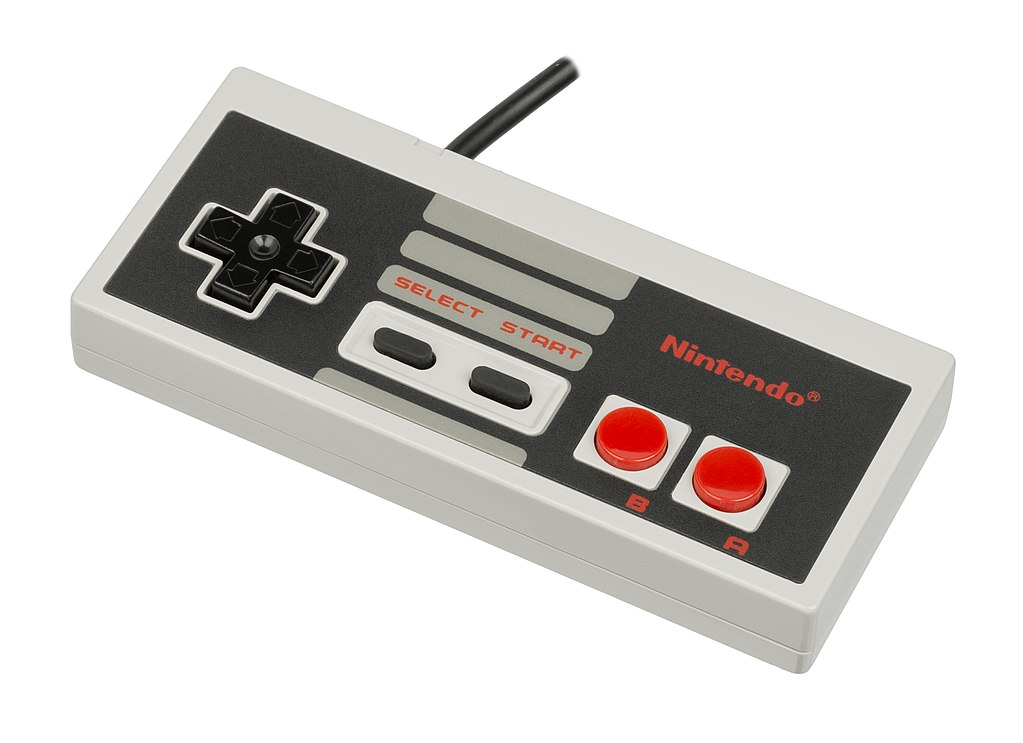
\includegraphics[width=0.6 \linewidth]{images/NEScontroller.jpg}
    \caption{An NES controller (Picture courtesy of Wikipedia)}
    \label{nesController}
\end{figure}

\begin{figure}[H]
    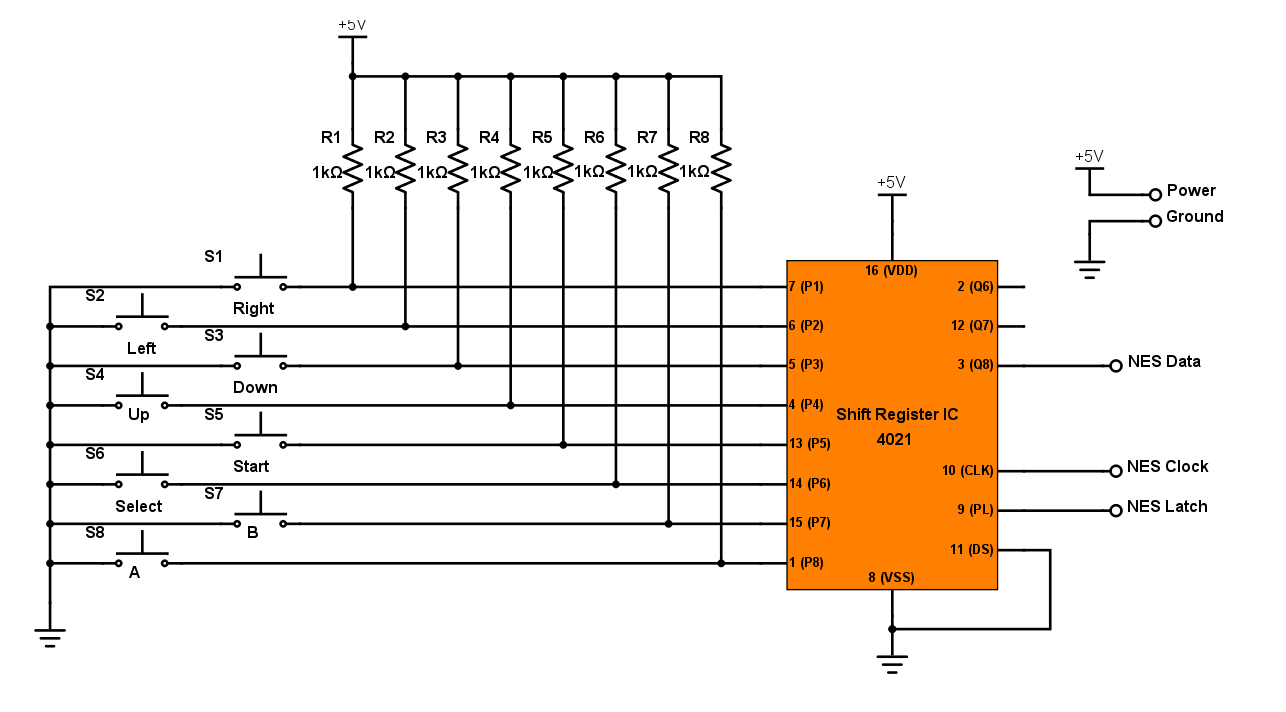
\includegraphics[width=0.8 \linewidth]{images/nesSchema.png}
    \caption{The buttons and shift register inside of an NES controller}
    \label{nesSchematic}
\end{figure}


\begin{figure}[H]
    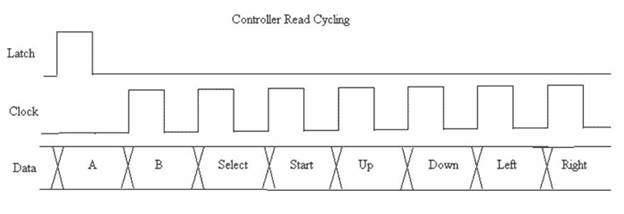
\includegraphics[width=0.8 \linewidth]{images/nesclock.jpg}
    \caption{One shift register worth of data, transmitted after pulsing the latch input high}
    \label{nesClock}
\end{figure}

An example of the NES controller decoder module was provided for us in the course materials, and a discussion of the code is included in the appendix of this document.

\subsection{Analog-to-Digital Converter}
The second input that we chose was an Analog-to-Digital Converter, also known as an ADC. After talking to a fellow classmate\footnote{Luke Goldsworthy} about how hard a time he was having accessing the DE10-Lite's on-board ADC (even with the help of teachers and TAs), our group decided to use an external one to interface with the DE10-Lite. An Arduino Nano converts an analog potentiometer's voltage from 0-5Vdc  to 0 to 1023 bits. The code running on the Arduino is included in the appendix section. 

\begin{figure}[H]
    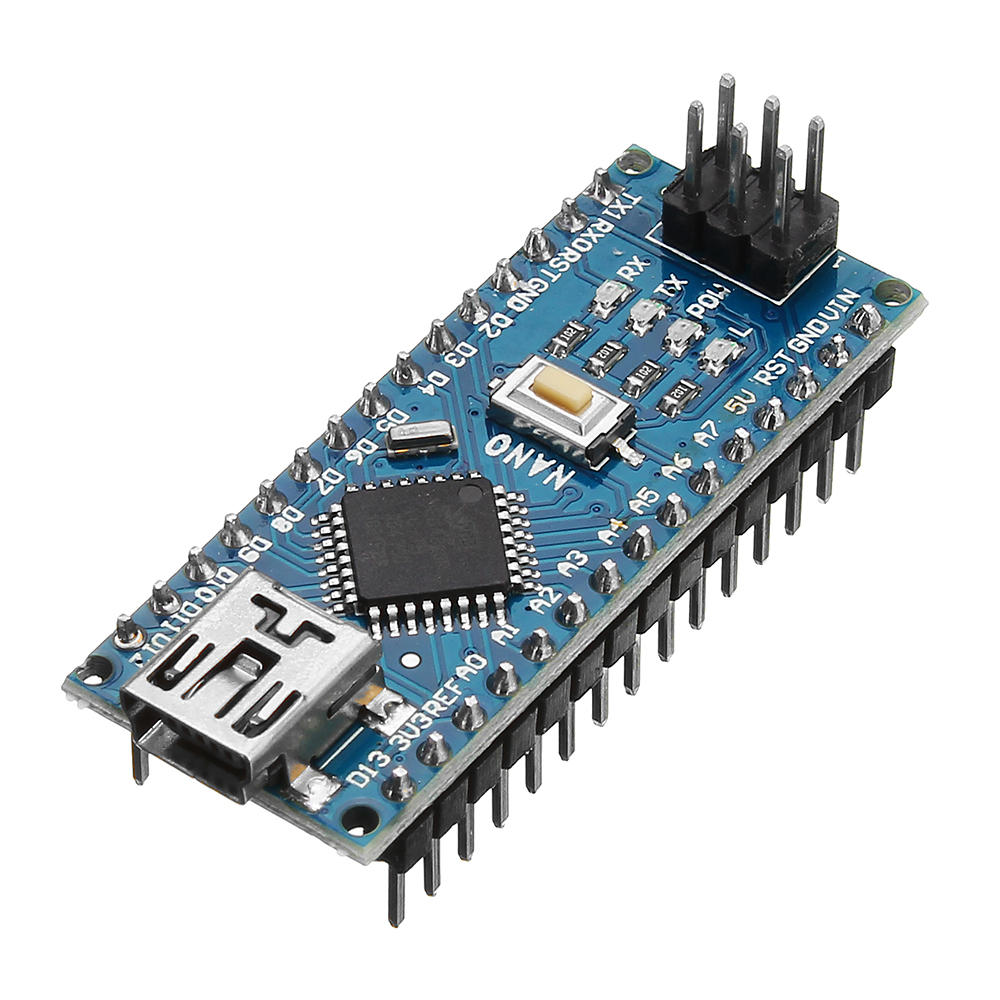
\includegraphics[width=0.6 \linewidth]{images/nano.jpg}
    \caption{The Arduino Nano includes a built-in ADC}
    \label{nano}
\end{figure}



\section{HDL Components}

\subsection{Top Module}

INSERT TOP MODULE DIAGRAM HERE

INSERT TOP MODULE DESCRIPTION HERE

\subsection{VGA Output}

\begin{figure}[H]
    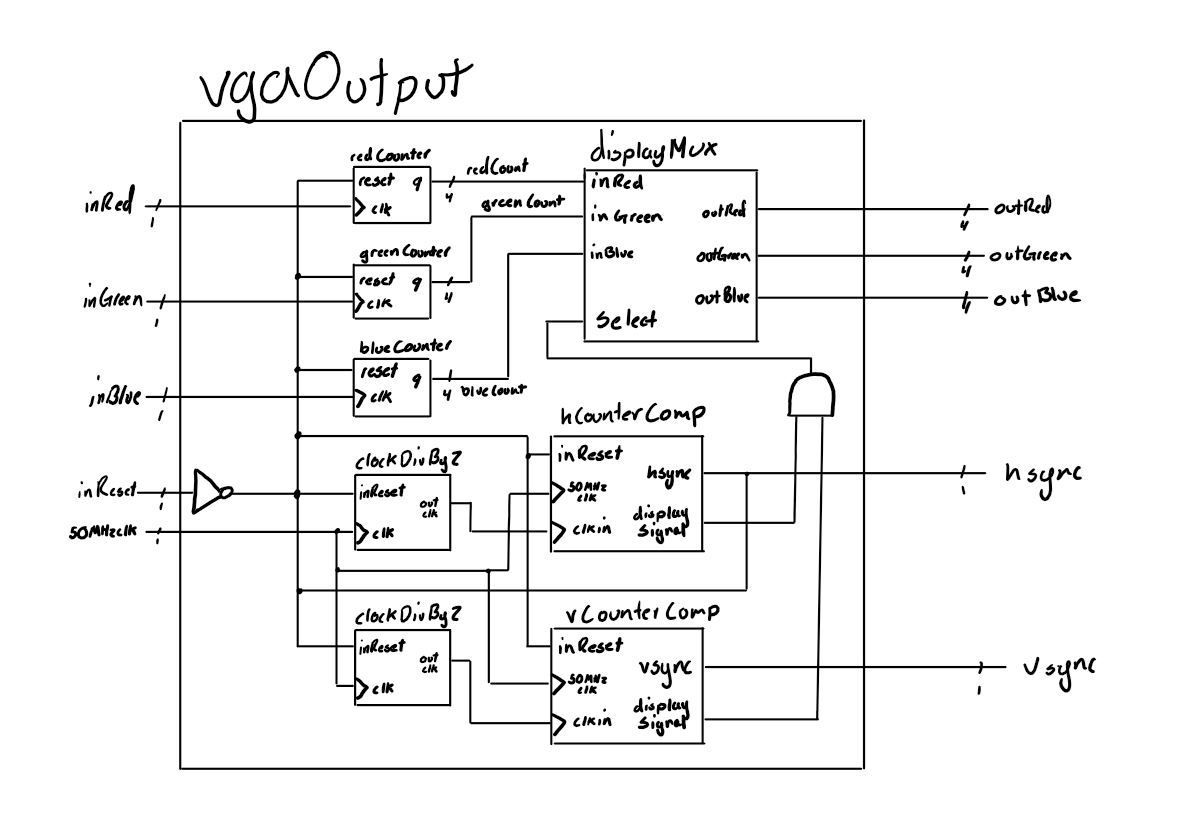
\includegraphics[width=0.8 \linewidth]{images/vgaOutput.JPG}
    \caption{VGA output module diagram}
    \label{vgaOutputDiagram}
\end{figure}


Input: The VGA module takes a 50MHz clock signal, a reset signal, and three button signals for the red, green, and blue inputs.

Output: The VGA module outputs a vSync and an hSync signal, and three 4-bit values for the red, green, and blue display colors.

Description: This module is designed to output a 640x480 resolution VGA signal, allowing it to display an RGB color value on a screen. The hSync signal tells a computer monitor how quickly to update each column of the screen, while the vSync signal tells it how quickly to update each row. The color inputs work by having each button press increment a 4-bit counter that goes to the appropriate color output.

\subsubsection{VGA hCounterComp}


Inputs: A 25MHz clock signal, a 50MHz clock signal, and a reset signal.
Outputs: The horizontal sync rate for the VGA output and a signal indicating that it is in the display area for the screen.

Description: The hCounterComp creates the hSync signal for the VGA driver, as well as indicating that the signal is within the display area so that the RGB values can be communicated to the screen. The hSync signal travels through the horizontal row of pixels on the screen, displaying color when appropriate.

\begin{figure}[H]
    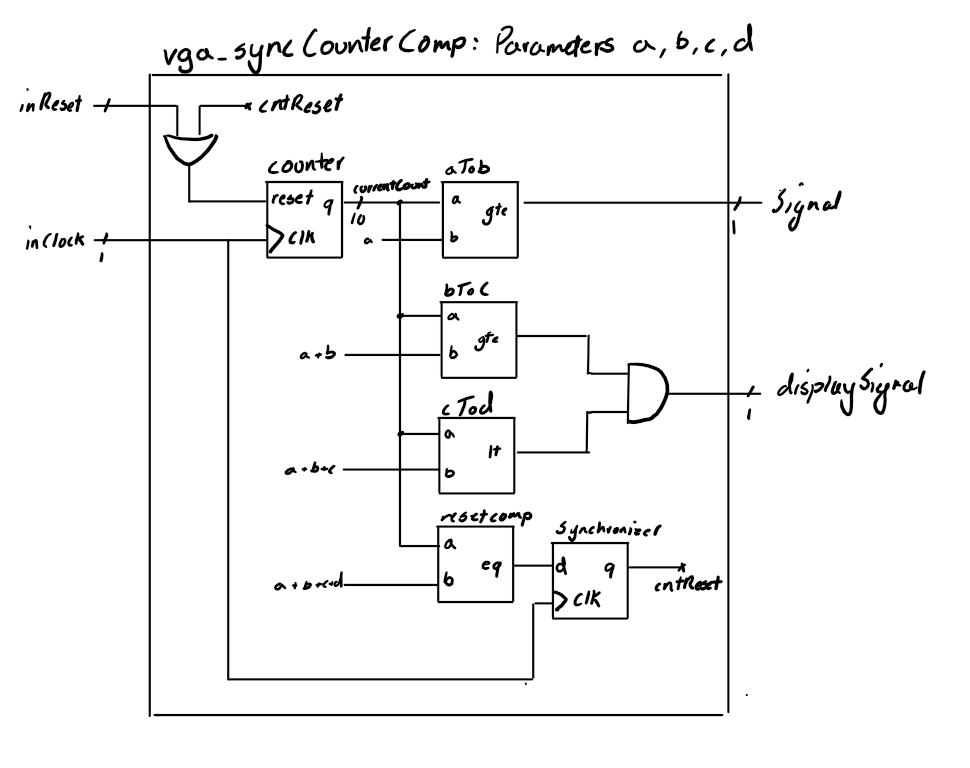
\includegraphics[width=0.8 \linewidth]{images/vga_syncCounterComp.JPG}
    \caption{VGA syncCounterComp module diagram}
    \label{vgaSyncCounterCompDiagram}
\end{figure}

\subsubsection{VGA vCounterComp}

INSERT DIAGRAM HERE

Inputs: The hSync signal as a clock, a 50MHz clock signal, and a reset signal.
Outputs: The vertical sync rate for the VGA output and a signal indicating that it is in the display area for the screen.

Description: The vCounterComp module generates the vSync signal for the VGA driver, which tells it when to move on to the next row of pixels, as well as telling it when it is within the displayable area.

\subsubsection{VGA counter}

\begin{figure}[H]
    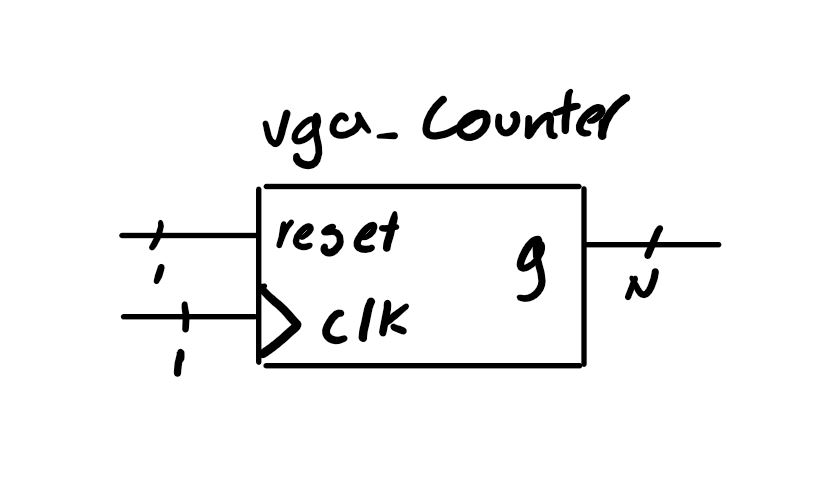
\includegraphics[width=0.8 \linewidth]{images/vga_counter.JPG}
    \caption{VGA counter module diagram}
    \label{vgaCounterDiagram}
\end{figure}

Inputs: A clock signal and a reset signal.
Outputs: An N-bit binary value.

Description: This counter adds one to its output value each rising clock edge.

\subsubsection{VGA displayMux}

\begin{figure}[H]
    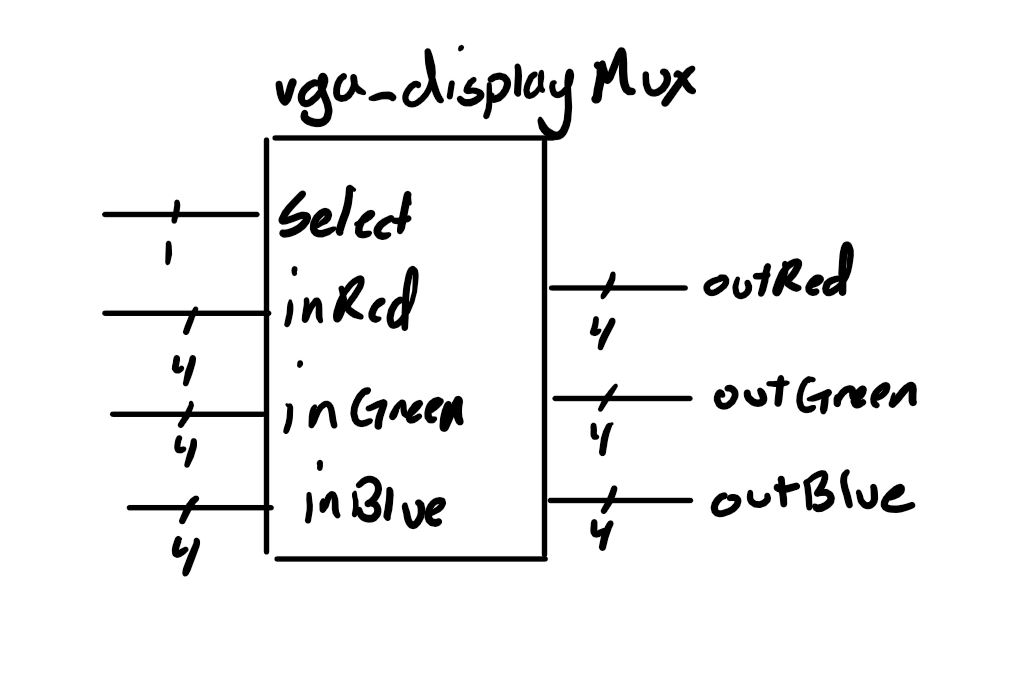
\includegraphics[width=0.8 \linewidth]{images/vga_displayMux.JPG}
    \caption{VGA displayMux module diagram}
    \label{vgaDisplayMuxDiagram}
\end{figure}

Inputs: A select signal and red, green, and blue binary input values.
Outputs: Either the inputted RGB values or 0 values.

Description: The VGA displayMux decides whether to send the inputted RGB values to the screen or not to, depending on whether or not we are within the displayable area, as given by the hSync and vSync modules.

\subsubsection{VGA comparator}

\begin{figure}[H]
    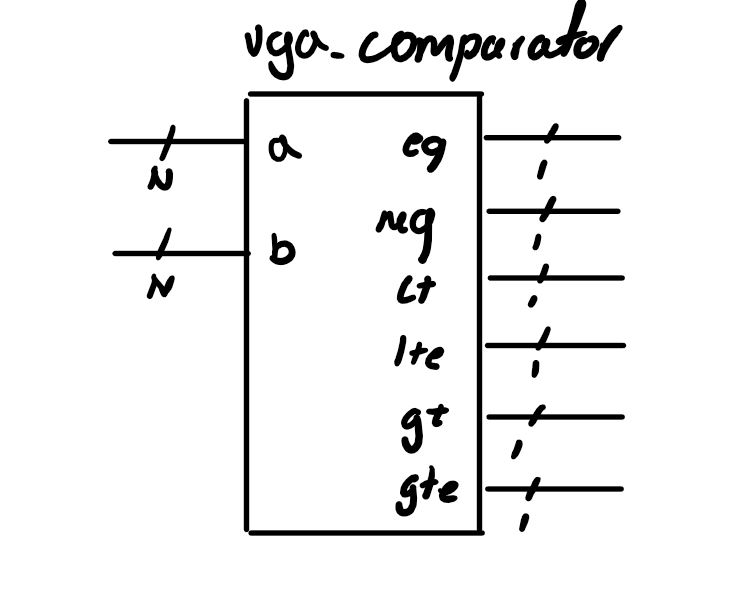
\includegraphics[width=0.8 \linewidth]{images/vga_comparator.JPG}
    \caption{VGA comparator module diagram}
    \label{vgaComparatorDiagram}
\end{figure}

Inputs: A select signal and red, green, and blue binary input values.
Outputs: Either the inputted RGB values or 0 values.

Description: The VGA displayMux decides whether to send the inputted RGB values to the screen or not to, depending on whether or not we are within the displayable area, as given by the hSync and vSync modules.

\subsubsection{VGA synchronizer}

\begin{figure}[H]
    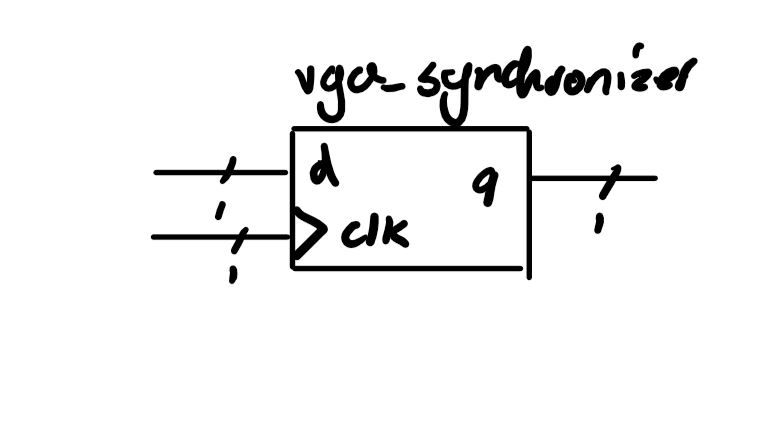
\includegraphics[width=0.8 \linewidth]{images/vga_synchronizer.JPG}
    \caption{VGA synchronizer module diagram}
    \label{vgaSynchronizerDiagram}
\end{figure}

Inputs: A clock signal and a 1-bit data value.
Outputs: A 1-bit data value.

Description: The synchronizer takes asynchronous inputs and syncs them to the clock edge.

\subsubsection{clockDivBy2}

\begin{figure}[H]
    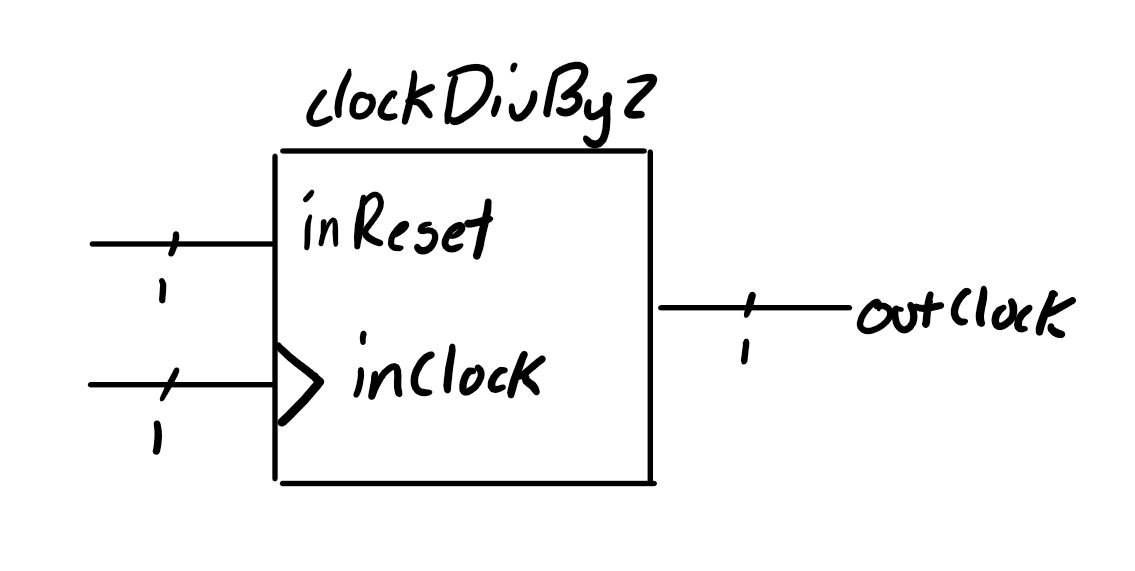
\includegraphics[width=0.8 \linewidth]{images/clockDivBy2.JPG}
    \caption{The clockDivBy2 module diagram}
    \label{clockDivBy2Diagram}
\end{figure}

Inputs: A clock signal and a reset signal.
Outputs: A clock signal half as fast as the input clock signal.

Description: This module takes in a clock input and divides its frequency by 2. For example, a 50MHz clock input would become a 25MHz clock input.

\subsection{Square Wave Generator}
Our square wave generator uses a simple algorithm to take a 10-bit array of data (from the analog input) and convert the value from $0-1023 $ bits to $\approx 100Hz $ to$ \approx 1600 Hz$. This range produces four octaves of the note G (i.e. a range from G2 to G6). This frequency range allows for the selection of many notes within the range of human hearing. 


\begin{equation}
1600/1123 \approx (10/7)
\end{equation}

The square wave generator's audio output is sent to a simple audio amplifier circuit (Seen in figure \ref{hardware} based on \href{https://www.instructables.com/id/Tales-From-the-Chip-LM386-Audio-Amplifier/}{this circuit} ), protecting the FPGAs output pins and providing more voltage. The amplifier then drives a simple 8$\Omega$ speaker. 

\subsection{Seven Segment Display}
Inputs: The seven segment display module (clock\_driver.sv) has an input for a 50 MHz clock signal, a reset, an enable, and start, left, right, up, down input signals from the NES controller.
Outputs: The clock_driver module has 6 7-bit outputs to connect to the seven segment display on the De10-Lite.

Description: This module is designed to have a working (and settable) 12 hour clock. If the user presses start they will be able to set the clock to any value. While setting the clock the user can navigate between seconds, minutes and hours. When a user is editing one of these states, the two corresponding seven segment displays will flash. When the user presses start again the time specified will start counting, as a clock should. The value that represents the hours on the clock will be a value between 0 and 11, but the displayed value for hours will be incremented by 1 in order to have the hours fall between 1 and 12.

\subsubsection{Seven Segment Display: clock}
\begin{figure}[H]
    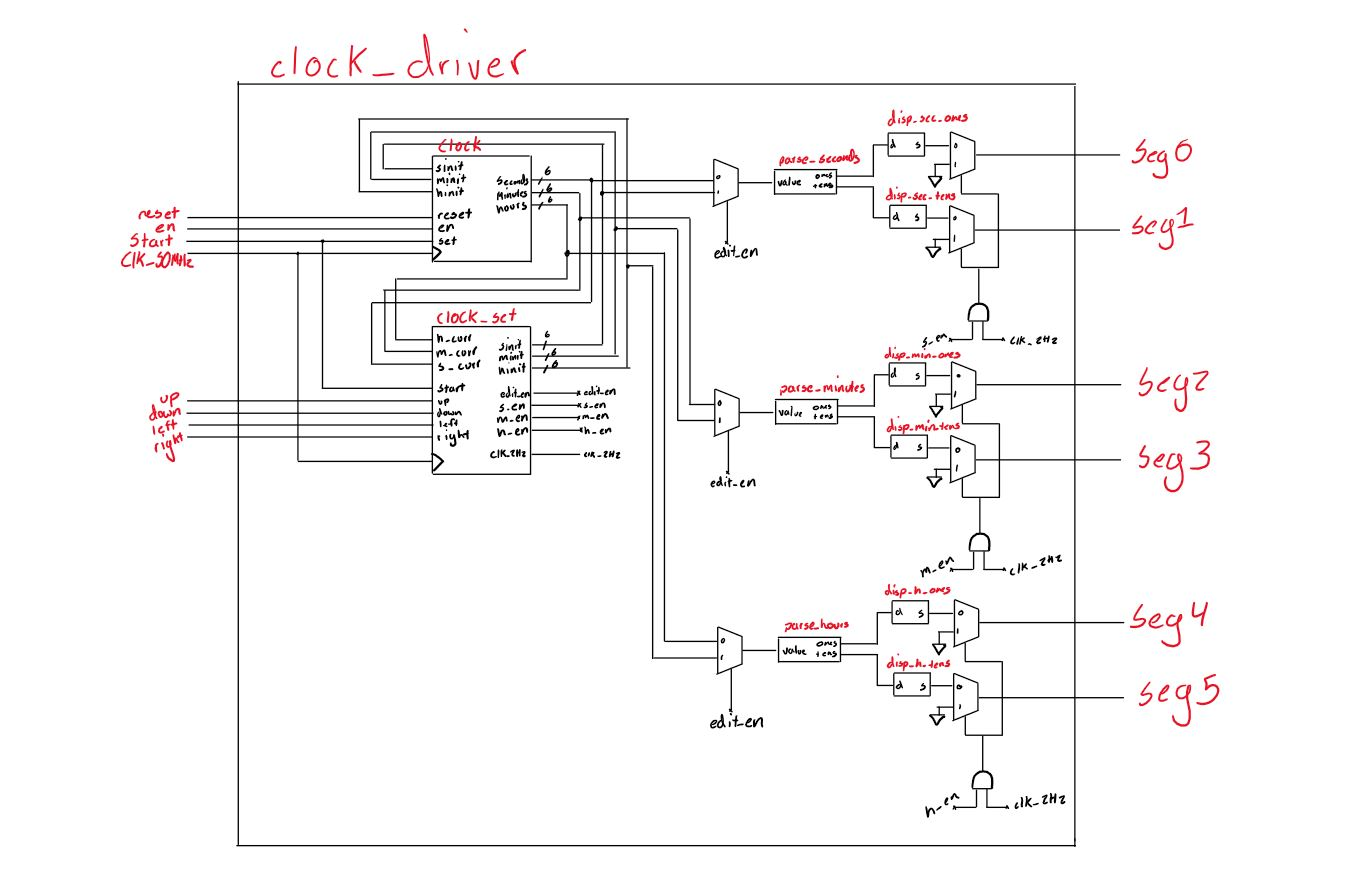
\includegraphics[width=0.8 \linewidth]{images/clock_driver.JPG}
    \caption{Block diagram for the clock_driver module}
    \label{clock_driver}
\end{figure}

Inputs: This module has an enable input and a reset input which will be driven by the select button on the NES controller. It has a clk input which will be assigned to the 50 MHz clock. It also has a set input, which will set the clock the the last three inputs, which are the initial values of seconds, minutes and hours.
Outputs: This module has three outputs, seconds, minutes and hours, which represent the value to be displayed on the clock.

Description: This module is a working and settable clock. If enable and set are HIGH and reset is LOW, the clock is running normally, counting up by seconds.

\subsubsection{Seven Segment Display: parser}
\begin{figure}[H]
    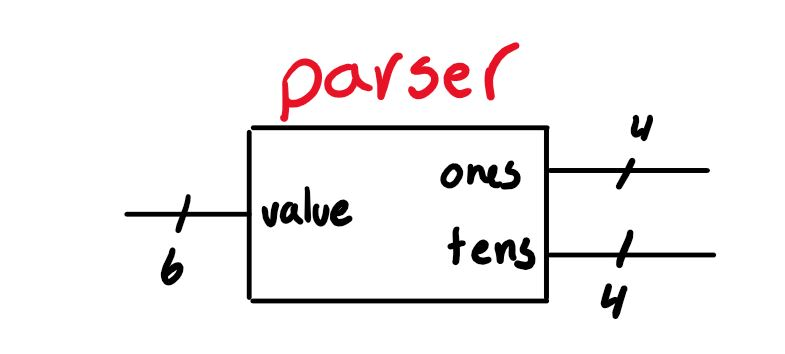
\includegraphics[width=0.8 \linewidth]{images/parser.JPG}
    \caption{Block diagram for the parser module}
    \label{parser}
\end{figure}

Inputs: This module has one input, the value to be parsed.
Outputs: This module has two outputs, the ones digit of value and the tens digit of value.

Description: The parser module takes a 6 bit input and separates it out into its two decimal, ones and tens, digits.

\subsubsection{Seven Segment Display: seven_seg_driver}
\begin{figure}[H]
    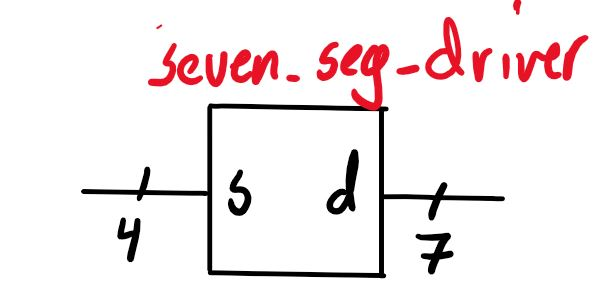
\includegraphics[width=0.8 \linewidth]{images/seven_seg_driver.JPG}
    \caption{Block diagram for the seven_seg_driver module}
    \label{seven_swg_driver}
\end{figure}

Inputs: This module has one input, d which is a 4 bit bus.
Outputs: This module has one output, s, a 7 bit bus.

Description: This module decodes a 4 bit binary value into a 7 bit bus that will drive an active low seven segment display.

\subsubsection{Seven Segment Display: clk_divider}
\begin{figure}[H]
    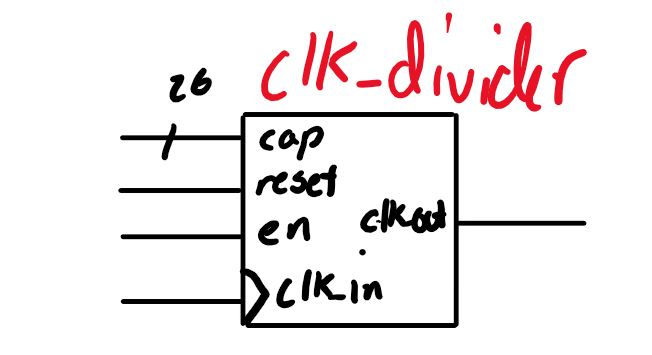
\includegraphics[width=0.8 \linewidth]{images/clk_divider.JPG}
    \caption{Block diagram for the clk_divider module}
    \label{clk_driver}
\end{figure}

Inputs: This module has four inputs, cap , reset, en and clk_in.
Outputs: This module has one output, clk_out.

Description: This module takes a clock signal as an input and when that clock signal has cycled the number of times specified by cap, it will toggle the clk_out signal, or it divides the clock signal.

\subsubsection{Seven Segment Display: clk_counter}
\begin{figure}[H]
    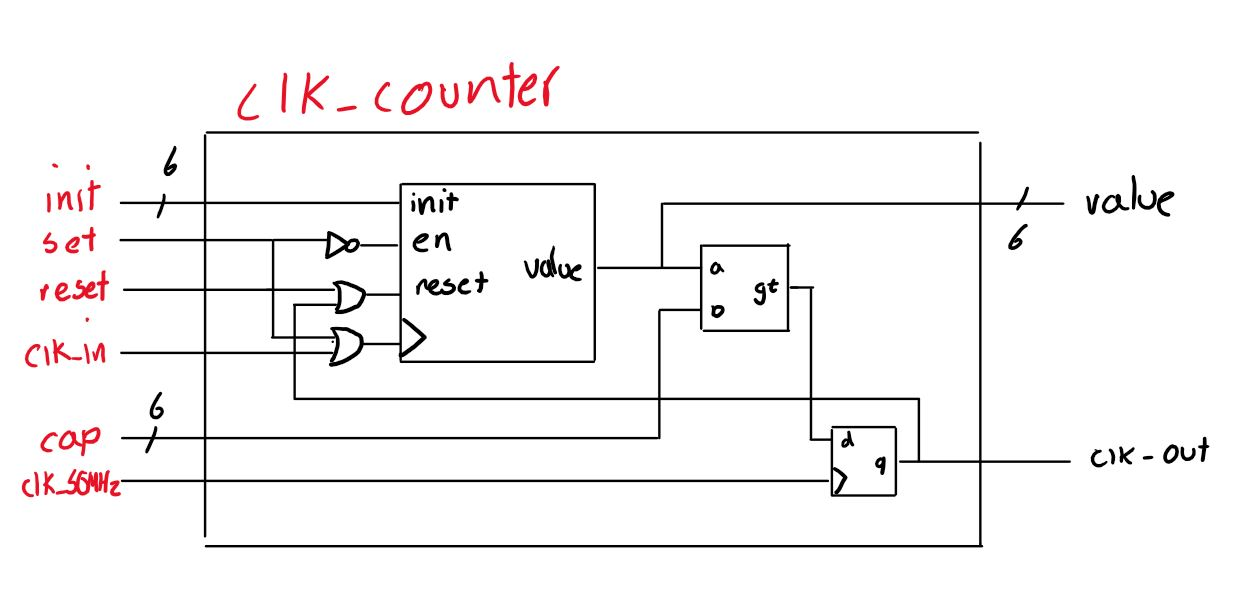
\includegraphics[width=0.8 \linewidth]{images/clk_counter.JPG}
    \caption{Block diagram for the clk_counter module}
    \label{clk_counter}
\end{figure}


Inputs: This module has six inputs, init, set, reset, clk_in, cap and clk_50MHz.
Outputs: This module has two outputs, value and clk_out.

Description: The clk_counter module, is a counter that increments on every rising edge of the clk_in. It then uses a comparator and synchronizer to see if that value exceeds the cap input, and if it does it resets to 0.

\subsubsection{Seven Segment Display: counter}
\begin{figure}[H]
    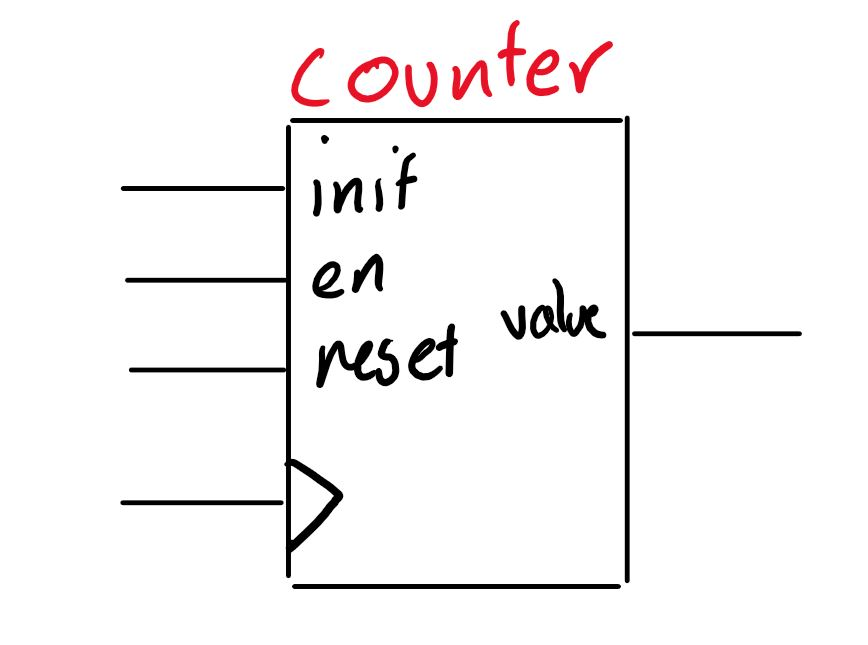
\includegraphics[width=0.8 \linewidth]{images/counter.JPG}
    \caption{Block diagram for the counter module}
    \label{counter}
\end{figure}

Inputs: The counter module takes 4 inputs, init, reset and clk_in.
Outputs: This module has one output, value.

Description: This module is a counter used for the seconds, minutes and hours of the clocks. If reset and en are LOW the count is set to equal the init input.

\subsubsection{Seven Segment Display: comp}
\begin{figure}[H]
    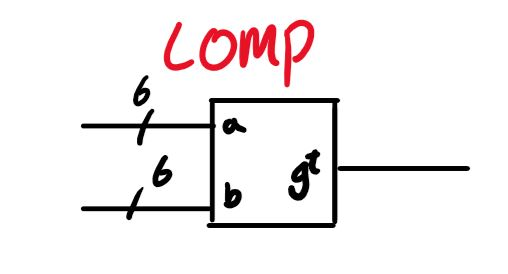
\includegraphics[width=0.8 \linewidth]{images/comp.JPG}
    \caption{Block diagram for the comp module}
    \label{comp}
\end{figure}

Inputs: The module comp, takes two inputs, a and b.
Outputs: It has one output, gt.

Description: Drives gt HIGH if a is greater than b.

\subsubsection{Seven Segment Display: sync}
\begin{figure}[H]
    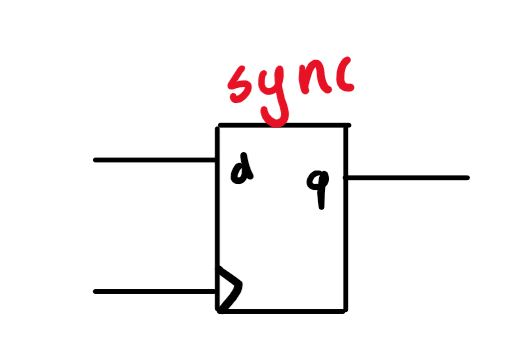
\includegraphics[width=0.8 \linewidth]{images/sync.JPG}
    \caption{Block diagram for the sync module}
    \label{sync}
\end{figure}

Inputs: Two inputs, d and clk.
Outputs: One output, q.

Description: Turns an asynchronous value into a synchronous value.

\subsubsection{Seven Segment Display: clock_set}
\begin{figure}[H]
    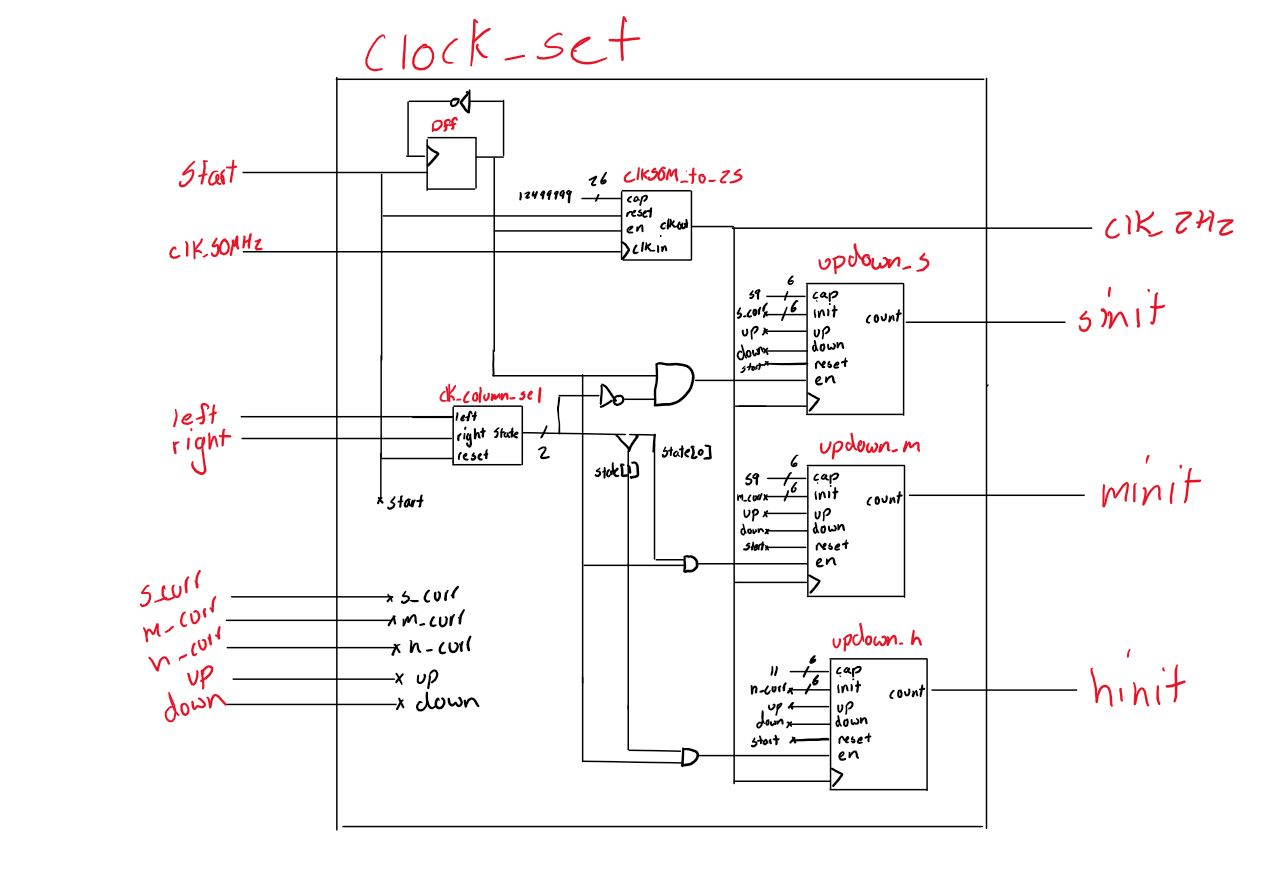
\includegraphics[width=0.8 \linewidth]{images/clock_set.JPG}
    \caption{Block diagram for the clock_set module}
    \label{clock_set}
\end{figure}

Inputs: clock_set has 9 inputs, start, clk_50MHz, left, right, up, down, s_curr, m_curr and h_curr.
Outputs: It has 4 outputs, clk_2Hz, sinit, minit and hinit.

Description: Clock set lets a user set the clock using a NES controller. When start is pulsed the clock goes into edit mode, the user can navigate through seconds, minutes and hours using the left or a button and the right or b button. The user can then add or subtract to the values, and when they find a desirable time to set the clock, they can push the start button again and it will send the outputs to the clock module.

\subsubsection{Seven Segment Display: clk_column_sel}
\begin{figure}[H]
    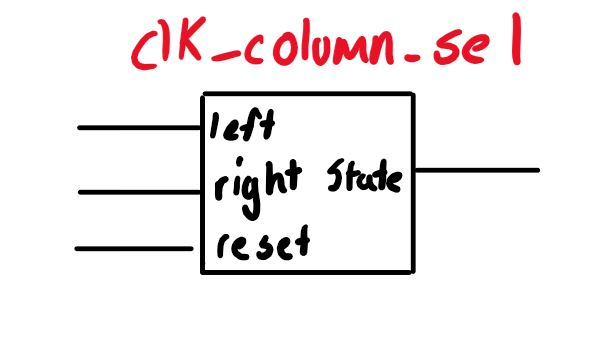
\includegraphics[width=0.8 \linewidth]{images/clk_column_sel.JPG}
    \caption{Block diagram for the clk_column_sel module}
    \label{clk_column_sel}
\end{figure}

Inputs:clk_column_sel has three inputs, left, right and reset. 
Outputs: This module has one output, which is the state of the system. 

Description:This module is a state machine that lets the use navigate through the seven segment displays and determines which column the user is editing by encoding seconds, minutes and hours into states. 

\subsubsection{Seven Segment Display: updowncounter}
\begin{figure}[H]
    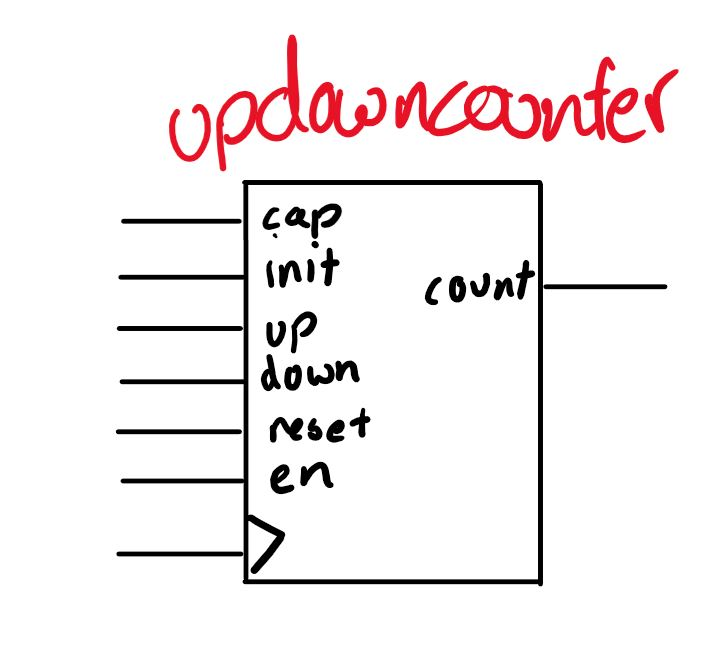
\includegraphics[width=0.8 \linewidth]{images/updowncounter.JPG}
    \caption{Block diagram for the updowncounter module}
    \label{updowncounter}
\end{figure}

Inputs: The updowncounter has seven inputs, cap, init, up, down, reset, en and a clock signal
Outputs: This module has one output, which is the current count stored in the register.

Description: This output is a counter that permits the user to count down or up. It is used to edit the clock values and will overflow both ways.

\section{Hardware}%%%%%%%%%%%%%%%

DISCUSSSSSSSSSSSSSSSSSSSSSSSS
\begin{figure}[H]
    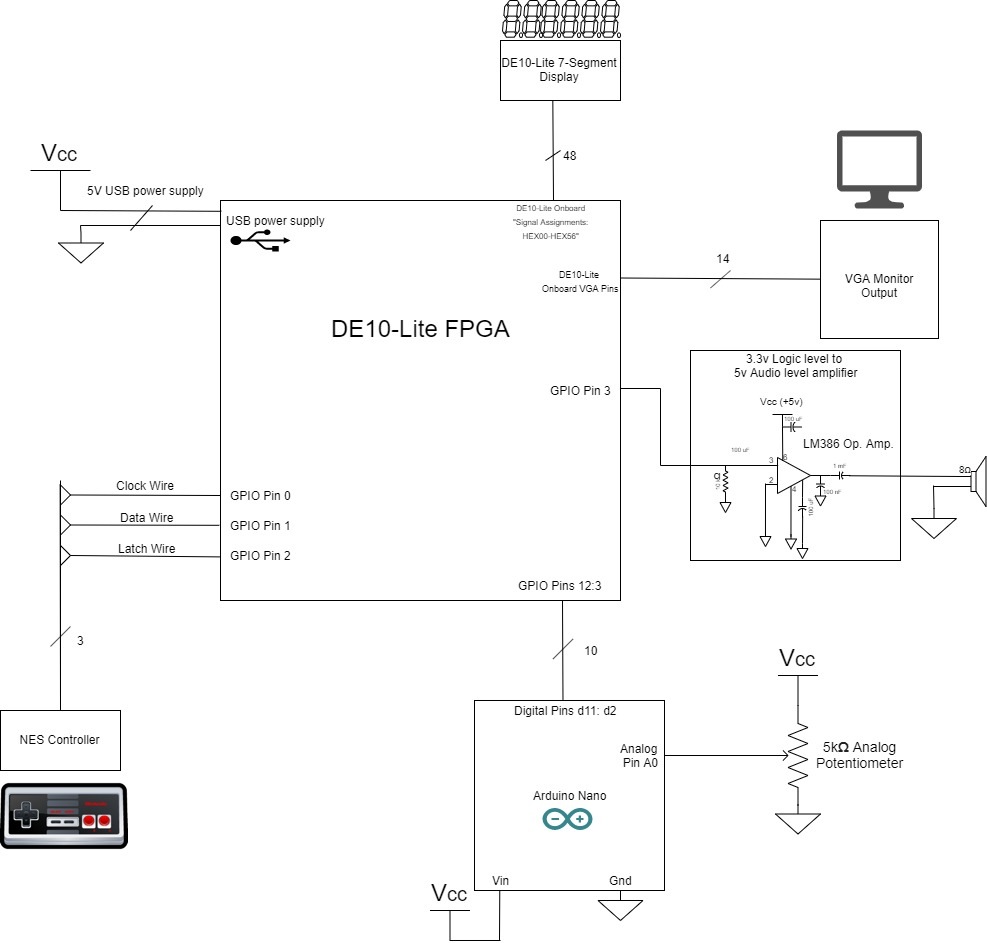
\includegraphics[width=0.8 \linewidth]{images/hardwareDiagram.jpg}
    \caption{ }
    \label{hardware}
\end{figure}

\section{Appendix}

\subsection{Source Code}%%%%%%%%%%%%%%%%%%%%%%%%%%%

\subsubsection{NES Controller Reader}
The NES reader module depends on four sub-modules. 
The "Counter4" module is just a resettable four-bit counter.
"NesLatchStateDecoder" receives the count from the "Counter4" counter and outputs a signal when all bits are zero. This signifies the latch signal which corresponds with the first high half of every eight clock cycles.
The "NesClockStateDecoder" module holds the combinational logic which controls the reader module's clock. 
Finally, the "NesDataReceiverDecoder" module reads data from the data wire at the negative edge of the controller's "Clock" signal and outputs a vector of these values. 


\begin{Verbatim}[tabsize = 4]
module NesReader(
  input logic dataYellow,
  input logic clock,
  input logic reset_n,
  output logic latchOrange,
  output logic clockRed,
  output logic up,
  output logic down,
  output logic left,
  output logic right,
  output logic start,
  output logic select,
  output logic a,
  output logic b
  );
  logic [3:0] count;

  Counter4 matt_i1(
    .clk               (clock), 
    .reset_n           (reset_n), 
    .count             (count)
  );

  NesClockStateDecoder matt_i2(
    .controllerState  (count), 
    .nesClock         (clockRed)
  );

  NesLatchStateDecoder matt_i3 (
    .controllerState  (count), 
    .nesLatch         (latchOrange)
  );

  NesDataReceiverDecoder matt_i4 (
    .dataYellow       (dataYellow), 
    .reset_n           (reset_n),
    .controllerState  (count), 
    .readButtons      ({a, b, select, start, up, down, left, right})
  );
endmodule

\end{Verbatim}

\begin{Verbatim}
module NesReader(
  input logic dataYellow,
  input logic clock,
  input logic reset_n,
  output logic latchOrange,
  output logic clockRed,
  output logic up,
  output logic down,
  output logic left,
  output logic right,
  output logic start,
  output logic select,
  output logic a,
  output logic b
  );
  logic [3:0] count;

  Counter4 matt_i1(
    .clk               (clock), 
    .reset_n           (reset_n), 
    .count             (count)
  );

  NesClockStateDecoder matt_i2(
    .controllerState  (count), 
    .nesClock         (clockRed)
  );

  NesLatchStateDecoder matt_i3 (
    .controllerState  (count), 
    .nesLatch         (latchOrange)
  );

  NesDataReceiverDecoder matt_i4 (
    .dataYellow       (dataYellow), 
    .reset_n           (reset_n),
    .controllerState  (count), 
    .readButtons      ({a, b, select, start, up, down, left, right})
  );
endmodule


module Counter4(
  input logic clk, reset_n,
  output logic [3:0] count);

  always_ff @ (posedge clk, negedge reset_n)
    if(!reset_n) count <= 4'b0;
    else count <= count + 1;
endmodule


module NesLatchStateDecoder(
  input logic [3:0] controllerState,
  output logic nesLatch);

  always_comb
    case(controllerState)
      4'h0: nesLatch = 1;
      default: nesLatch = 0;
    endcase
endmodule


module NesClockStateDecoder(
  input logic [3:0] controllerState,
  output logic nesClock);

  always_comb
    case (controllerState)
      4'h2: nesClock = 1;
      4'h4: nesClock = 1;
      4'h6: nesClock = 1;
      4'h8: nesClock = 1;
      4'ha: nesClock = 1;
      4'hC: nesClock = 1;
      4'hE: nesClock = 1;
      default: nesClock = 0;
    endcase
endmodule


module Counter4(
  input logic clk, reset_n,
  output logic [3:0] count);

  always_ff @ (posedge clk, negedge reset_n)
    if(!reset_n) count <= 4'b0;
    else count <= count + 1;
endmodule


module NesLatchStateDecoder(
  input logic [3:0] controllerState,
  output logic nesLatch);

  always_comb
    case(controllerState)
      4'h0: nesLatch = 1;
      default: nesLatch = 0;
    endcase
endmodule


module NesClockStateDecoder(
  input logic [3:0] controllerState,
  output logic nesClock);

  always_comb
    case (controllerState)
      4'h2: nesClock = 1;
      4'h4: nesClock = 1;
      4'h6: nesClock = 1;
      4'h8: nesClock = 1;
      4'ha: nesClock = 1;
      4'hC: nesClock = 1;
      4'hE: nesClock = 1;
      default: nesClock = 0;
    endcase
endmodule


module NesDataReceiverDecoder(
  input logic dataYellow,
  input logic reset_n,
  input logic [3:0] controllerState,
  output logic [7:0] readButtons); 

  always_ff @ (posedge controllerState[0], negedge reset_n)
    if(!reset_n) readButtons <= 8'b0;
    else case(controllerState[3:0])
      4'h1: readButtons[7] <= dataYellow;	//a button
      4'h3: readButtons[6] <= dataYellow;	//b button
      4'h5: readButtons[5] <= dataYellow;	//select button
      4'h7: readButtons[4] <= dataYellow;	//start button
      4'h9: readButtons[3] <= dataYellow;	//up button
      4'hB: readButtons[2] <= dataYellow;	//down button
      4'hD: readButtons[1] <= dataYellow;	//left button
      4'hF: readButtons[0] <= dataYellow;	//right button
      default: readButtons <= readButtons;
    endcase
endmodule
\end{Verbatim}

\subsubsection{ADC}
The following code is written in Arduino C and uploaded to an Arduino Nano microcontroller. 

\begin{Verbatim}[tabsize = 4]

int analogPin = A0;	// the potentiometer's analog voltage

int d2 = 2;				// the first output bit
int d3 = 3;
int d4 = 4;
int d5 = 5;
int d6 = 6;
int d7 = 7;
int d8 = 8;
int d9 = 9;				
int d10 = 10;
int d11 = 11;// the last (most significant) output bit

void setup() 
{
  pinMode(analogPin, INPUT);              // Potentiometer input pin
  
  pinMode(d2, OUTPUT);           //Indicates the pinmode of selected pin
  pinMode(d3, OUTPUT);           //Indicates the pinmode of selected pin
  pinMode(d4, OUTPUT);           //Indicates the pinmode of selected pin
  pinMode(d5, OUTPUT);           //Indicates the pinmode of selected pin
  pinMode(d6, OUTPUT);           //Indicates the pinmode of selected pin
  pinMode(d7, OUTPUT);           //Indicates the pinmode of selected pin
  pinMode(d8, OUTPUT);           //Indicates the pinmode of selected pin
  pinMode(d9, OUTPUT);           //Indicates the pinmode of selected pin
  pinMode(d10, OUTPUT);           //Indicates the pinmode of selected pin
  pinMode(d11, OUTPUT);           //Indicates the pinmode of selected pin
}

void loop() 
{
  int value = analogRead(analogPin);
  int pinArray[10];
  bool bitArray[10];
  for (int i=0; i<=9; i++)
  {
    pinArray[i] = i+2;			// assigns outputs 2-11
    if (bitRead(value,i))
       {digitalWrite( pinArray[i],HIGH);}	//accesses the correct pin and writes HIGH
    else
       {digitalWrite( pinArray[i],LOW);}		//accesses the correct pin and writes LOW
  }
}
\end{Verbatim}

\subsubsection{Square Wave Generator}

\begin{Verbatim}[tabsize=4]

module periodTime(input logic clk,
					input logic [9:0] data,
					output logic q);
					
int compareNumber;
int count;

always_ff @(negedge q)
	begin
		compareNumber = (data + 100)*(10/7);
		if (count >= compareNumber)
		count <= 0;
	end
		
always_ff @(posedge clk)
	begin
			count <= count +1;
	end

always_comb
	begin
			if( count < compareNumber)				
				q = (count > compareNumber/2); 	//assigns output duty cycle 50% with initial low
			else 
				q = 0;
	end

endmodule
\end{Verbatim}

\subsubsection{VGA Output}

\begin{Verbatim}
module vgaOutput
		(input clock50MHz,
		 input inReset,
		 input inRed,
		 input inGreen,
		 input inBlue,
		 output hSync,
		 output vSync,
		 output [3:0] outRed, outGreen, outBlue);
	
	vga_counter #(.N(4)) redCounter (
		.clk(inRed),
		.reset(inReset),
		.q(redCount)
	);
	
	vga_counter #(.N(4)) greenCounter (
		.clk(inGreen),
		.reset(inReset),
		.q(greenCount)
	);
	
	vga_counter #(.N(4)) blueCounter (
		.clk(inBlue),
		.reset(inReset),
		.q(blueCount)
	);

	clockDivBy2 clockDivider(
		.clock50MHz(clock50MHz),
		.inReset(~inReset),
		.outClock(clock25MHz)
	);
	
	vga_hCounterComp #(.a(10'd96), .b(10'd48), .c(10'd640), .d(10'd16)) hSyncCounter (
		.inClock(clock25MHz),
		.clock50MHz(clock50MHz),
		.inReset(~inReset),
		.signal(hSync),
		.displaySignal(hSignal)
	);
	
	clockDivBy2 syncDivider(
		.clock50MHz(hSync),
		.inReset(~inReset),
		.outClock(hClock)
	); 
	
	vga_vCounterComp #(.a(10'd2), .b(10'd33), .c(10'd480), .d(10'd10)) vSyncCounter (
		.inClock(hClock),
		.clock50MHz(clock50MHz),
		.inReset(~inReset),
		.signal(vSync),
		.displaySignal(vSignal)
	);
	
	vga_displayMux display (
		.select(hSignal & vSignal),
		.inRed(redCount),
		.inGreen(greenCount),
		.inBlue(blueCount),
		.outRed(outRed),
		.outGreen(outGreen),
		.outBlue(outBlue)
	);

endmodule
\end{Verbatim}

\subsubsection{VGA hCounterComp}

\begin{Verbatim}
module vga_hCounterComp #(parameter a = 10, b = 10, c = 10, d = 10)
		(input inClock,
		 input clock50MHz,
		 input inReset,
		 output signal,
		 output displaySignal);
		 
	logic [9:0] currentCount;

	vga_counter #(.N(10)) count1 (
		.clk(inClock),
		.reset(cntReset | inReset),
		.q(currentCount)
	);
	
	vga_comparator #(.N(10)) aTob (
		.a(currentCount),
		.b(a),
		.gte(signal)
	);
	
	vga_comparator #(.N(10)) bToc (
		.a(currentCount),
		.b(a + b),
		.gte(disp1)
	);
	
	vga_comparator #(.N(10)) cToD (
		.a(currentCount),
		.b(a + b + c),
		.lt(disp2)
	);
	
	vga_comparator #(.N(10)) reset (
		.a(currentCount),
		.b(a + b + c + d),
		.eq(compSignal)
	);
	
	vga_synchronizer sync1 (
		.clk(clock50MHz),
		.d(compSignal),
		.q(cntReset)
	);
	
	assign displaySignal = disp1 & disp2;

endmodule
\end{Verbatim}

\subsubsection{VGA vCounterComp}

\begin{Verbatim}
module vga_vCounterComp #(parameter a = 10, b = 10, c = 10, d = 10)
		(input inClock,
		 input clock50MHz,
		 input inReset,
		 output signal,
		 output displaySignal);
		 
	logic [9:0] currentCount;

	vga_counter #(.N(10)) count1 (
		.clk(inClock),
		.reset(cntReset | inReset),
		.q(currentCount)
	);
	
	vga_comparator #(.N(10)) aTob (
		.a(currentCount),
		.b(a),
		.gte(signal)
	);
	
	vga_comparator #(.N(10)) bToc (
		.a(currentCount),
		.b(a + b),
		.gte(disp1)
	);
	
	vga_comparator #(.N(10)) cToD (
		.a(currentCount),
		.b(a + b + c),
		.lt(disp2)
	);
	
	vga_comparator #(.N(10)) reset (
		.a(currentCount),
		.b(a + b + c + d),
		.eq(compSignal)
	);
	
	vga_synchronizer sync1 (
		.clk(clock50MHz),
		.d(compSignal),
		.q(cntReset)
	);
	
	assign displaySignal = disp1 & disp2;

endmodule
\end{Verbatim}

\subsubsection{VGA counter}

\begin{Verbatim}
module vga_counter #(parameter N = 4)
		(input logic clk,
		 input logic reset,
		 output logic [N-1:0] q);

	always_ff @(posedge clk, posedge reset) begin
		if (reset)	q <= 0;
		else			q <= q + 1;
	end

endmodule
\end{Verbatim}

\subsubsection{VGA displayMux}

\begin{Verbatim}
module vga_counter #(parameter N = 4)
		(input logic clk,
		 input logic reset,
		 output logic [N-1:0] q);

	always_ff @(posedge clk, posedge reset) begin
		if (reset)	q <= 0;
		else			q <= q + 1;
	end

endmodule
\end{Verbatim}

\subsubsection{VGA comparator}

\begin{Verbatim}
module vga_comparator #(parameter N = 1)
		(input logic [N-1:0] a, b,
		 output logic eq, neq, lt, lte, gt, gte);

	assign eq	= (a == b);
	assign neq	= (a != b);
	assign lt	= (a < b);
	assign lte	= (a <= b);
	assign gt	= (a > b);
	assign gte	= (a >= b);

endmodule
\end{Verbatim}

\subsubsection{VGA synchronizer}

\begin{Verbatim}
module vga_synchronizer
		(input logic clk,
		 input logic d,
		 output logic q);

	logic n1;
	
	always_ff @(posedge clk)
		begin
			n1 <= d;
			q <= n1;
		end

endmodule
\end{Verbatim}

\subsubsection{clockDivBy2}

\begin{Verbatim}
module clockDivBy2
	(input clock50MHz,
	 input inReset,
	 output reg outClock);

	always @(posedge clock50MHz) begin
		if (inReset)
			  outClock <= 1'b0;
		else
			  outClock <= ~outClock;
	end

endmodule
\end{Verbatim}

\subsubsection{Seven Segment Display: clock_driver}
\begin{Verbatim}
module clock_driver(input logic clk_50MHz,
                    input logic start, up, down, left, right,
                    input logic reset,
						  input logic en,
						  output logic [6:0] Seg0, Seg1, Seg2, Seg3, Seg4, Seg5);
						
	logic edit_en, s_en, m_en, h_en;
	
	logic clk_2Hz;
	
	logic [6:0] s_seg_ones, s_seg_tens, m_seg_ones, m_seg_tens, h_seg_ones, h_seg_tens;
	logic [5:0] clk_hours, clk_minutes, clk_seconds, hinit, minit, sinit;
	logic [3:0] sec_ones, sec_tens, min_ones, min_tens, h_ones, h_tens;
	
	clock clk (
	   
		.hinit              (hinit),
		.minit              (minit),
		.sinit              (sinit),
		.en                    (en),
		.set              (start),
		.reset              (reset),
		.clk_50MHz      (clk_50MHz),
		.hours          (clk_hours),
		.minutes      (clk_minutes),
		.seconds      (clk_seconds)
	
	);
	
	clock_set clk_set (
	   
		.start                    (start),	
		.up                          (up),        
		.down                      (down),
		.left                      (left), 
		.right                    (right),
      .h_curr               (clk_hours), 
		.m_curr             (clk_minutes), 
		.s_curr             (clk_seconds),       
      .clk_50MHz            (clk_50MHz),
		.edit_en                (edit_en), 
		.h_en                      (h_en), 
		.m_en                      (m_en), 
		.s_en                      (s_en),
		.hours                    (hinit), 
		.minutes                  (minit), 
		.seconds                  (sinit),
		.clk_2Hz                (clk_2Hz)
	
	);
	
	
	
	parser #(6) parse_seconds(
	   
		.value    (edit_en ? sinit : clk_seconds),
	   .ones                          (sec_ones),
		.tens                          (sec_tens)  
	
	);
	
	seven_seg_driver disp_sec_ones(
	
	   .data         (sec_ones),
		.segments    (s_seg_ones)
	
	);
	
	assign Seg0 = (s_en & clk_2Hz) ? 1 : s_seg_ones; 
	
	seven_seg_driver disp_sec_tens(
	
	   .data         (sec_tens),
		.segments   (s_seg_tens)
	
	);
	
	assign Seg1 =  (s_en & clk_2Hz) ? 1 : s_seg_tens;  
	
	parser #(6) parse_minutes(
	   
		.value    (edit_en ? minit : clk_minutes),
	   .ones                      (min_ones),
		.tens                      (min_tens)
	
	);
	
	
	seven_seg_driver disp_min_ones(
	
	   .data             (min_ones),
		.segments       (m_seg_ones)
	
	);
	
	assign Seg2 = (m_en & clk_2Hz) ? 1 : m_seg_ones; 
	
	seven_seg_driver disp_min_tens(
	
	   .data             (min_tens),
		.segments       (m_seg_tens)
	
	);
	
	assign Seg3 =  (m_en & clk_2Hz) ? 1 : m_seg_tens; 
	
	parser #(6) parse_hours(
	   
		.value  (edit_en ? hinit + 1 : clk_hours + 1),
	   .ones                            (h_ones),
		.tens                            (h_tens)
	
	);
	
	seven_seg_driver disp_h_ones(
	
	   .data               (h_ones),
		.segments       (h_seg_ones)
	
	);
	
	assign Seg4 = (h_en & clk_2Hz) ? 1 : h_seg_ones; 
	
	seven_seg_driver disp_h_tens(
	
	   .data               (h_tens),
		.segments       (h_seg_tens)
	
	);
	
	assign Seg5 =  (h_en & clk_2Hz) ? 1 : h_seg_tens; 
	 

endmodule 
\end{Verbatim}

\subsubsection{Seven Segment Display: clock}
\begin{Verbatim}
module clock(input logic      [5:0] hinit, minit, sinit,
             input logic                 en, set, reset,
				 input logic                      clk_50MHz,
				 output logic [5:0] hours, minutes, seconds);
   
	logic clk_1Hz, clk_seconds, clk_minutes;
	
	
	clk_divider clk50M_to_1(
	
      .cap       (26'd24999999),
		.clk_in       (clk_50MHz),
		.reset            (reset),
		.en                  (en),
		.clk_out        (clk_1Hz)
	
	);
	
	clk_counter seconds_counter(
	
	   .init             (sinit),
	   .clk_in          (clk_1Hz),
		.clk_50MHz     (clk_50MHz),
		.cap               (6'd59),
		.reset             (reset),
		.set                 (set),
		.value           (seconds),
		.clk_out     (clk_seconds)
	
	);
	
	clk_counter minutes_counter(
	
	   .init              (minit),
	   .clk_in      (clk_seconds),
		.clk_50MHz     (clk_50MHz),
		.cap               (6'd59),
		.reset             (reset),
		.set                 (set),
		.value           (minutes),
		.clk_out     (clk_minutes)
	
	);

   clk_counter hours_counter(
	
	   .init              (hinit),
	   .clk_in      (clk_minutes),
		.clk_50MHz     (clk_50MHz),
		.cap               (6'd11),
		.reset             (reset),
		.set                 (set),
		.value             (hours)
	
	);

endmodule 
\end{Verbatim}

\subsubsection{Seven Segment Display: parser}
\begin{Verbatim}
module parser #(N = 8)
               (input logic [N-1:0]     value,
					 output logic [3:0] ones, tens);
	
	 assign ones = value % 4'd10;				
	 assign tens = (value - ones) / 4'd10;
					
endmodule 
\end{Verbatim}

\subsubsection{Seven Segment Display: seven_seg_driver}
\begin{Verbatim}
module seven_seg_driver(input logic [3:0] data,
                        output logic [6:0] segments);
								
   always_comb
	   case(data)
		   //                        abc defg
			0:         segments = 7'b100_0000;
			1:         segments = 7'b111_1001;
			2:         segments = 7'b010_0100;
			3:         segments = 7'b011_0000;
			4:         segments = 7'b001_1001;
			5:         segments = 7'b001_0010;
			6:         segments = 7'b000_0010;
			7:         segments = 7'b111_1000;
			8:         segments = 7'b000_0000;
			9:         segments = 7'b001_1000;
			default:   segments = 7'b111_1111;
		endcase
	
endmodule 
\end{Verbatim}

\subsubsection{Seven Segment Display: clk_divider}
\begin{Verbatim}
module clk_divider(input logic     clk_in,
                   input logic [25:0] cap,
					    input logic  reset, en,
						 output logic   clk_out);
   							
	logic [25:0] count;						
   
	
	always_ff@(posedge clk_in, posedge reset)
	   if(reset) 
		   begin
			   clk_out <= 0;
				count <= 0;
			   
			end
		else if(count > cap)
		   begin
			   clk_out <= ~clk_out;
				count <= 0;
			
			end
      else if(en) count <= count + 1;
	
    

endmodule 

\end{Verbatim}

\subsubsection{Seven Segment Display: clk_counter}
\begin{Verbatim}
module clk_counter(input logic [5:0]          init, cap,
                   input logic               set, reset,
						 input logic        clk_in, clk_50MHz,
						 output logic [5:0]             value,
						 output logic                 clk_out);

   logic gt;
	
	counter clk_count(
	   
		.init                (init),
		.en                  (~set),
		.reset    (reset | clk_out),
		.clk         (clk_in | set),
		.count              (value)
	
	);
	
	
	comp comparator(
	   
		.a    (value),   
		.b      (cap),
		.gt      (gt)
	
	);
	

	sync synchronizer(
	
	   .clk  (clk_50MHz),
		.d           (gt),
		.q      (clk_out)
	
	);
	

endmodule 
\end{Verbatim}

\subsubsection{Seven Segment Display: counter}
\begin{Verbatim}
module counter(input logic [5:0]           init,
               input logic            en, reset,
					input logic                  clk,
					output logic [5:0]         count);
					
   always_ff@(posedge clk, posedge reset)
	   if(reset) count <= 0;
		else if(en) count <= count + 1;
		else count <= init;



endmodule 
\end{Verbatim}

\subsubsection{Seven Segment Display: comp}
\begin{Verbatim}
module comp(input logic [5:0] a, b,
            output logic gt);
 
   assign gt = (a > b);

endmodule 
\end{Verbatim}

\subsubsection{Seven Segment Display: sync}
\begin{Verbatim}
module sync(input logic  clk,
            input logic    d,
			   output logic   q);


	logic n;
	
	always_ff@(posedge clk) 
	   begin
	   
		   n <= d;
		   q <= n;
		
	   end
	   

endmodule 
\end{Verbatim}

\subsubsection{Seven Segment Display: clock_set}
\begin{Verbatim}
module clock_set(input logic start, up, down, left, right,
                 input logic [5:0] h_curr, m_curr, s_curr,
                 input logic clk_50MHz,
					  output logic edit_en, h_en, m_en, s_en,
					  output logic [5:0] hours, minutes, seconds,
					  output logic clk_2Hz);
					  
   
	logic [1:0] state_sel;

	
	
	clk_divider clk50M_to_2(
	
      .cap       (26'd12499999),
		.clk_in       (clk_50MHz),
		.reset            (start),
		.en             (edit_en),
		.clk_out        (clk_2Hz)
	
	);
	
	
	clk_column_sel clk_nav(
	   .left      (left),
		.right     (right),
		.reset      (start),
		.state    (state_sel)
	
	);
	
	
	
	assign s_en = edit_en & (~state_sel[0] & ~state_sel[1]);
	assign m_en = edit_en & state_sel[0];
	assign h_en = edit_en & state_sel[1];
	
	
	updowncounter s_count(
	
      .up             (up),
		.down         (down),
	   .en           (s_en),
		.clk_in    (clk_2Hz),
	   .reset       (start),
		.cap         (6'd59),
		.init       (s_curr),
		.count     (seconds)
	
	);
	
	updowncounter m_count(
	
      .up             (up),
		.down         (down),
	   .en           (m_en),
		.clk_in    (clk_2Hz),
	   .reset       (start),
		.cap         (6'd59),
		.init       (m_curr),
		.count     (minutes)
	
	);
	
	updowncounter h_count(
	
      .up             (up),
		.down         (down),
	   .en           (h_en),
		.clk_in    (clk_2Hz),
	   .reset       (start),
		.cap         (6'd11),
		.init       (h_curr),
		.count       (hours)
	
	);
	
	
	
					  
   

					  
   always_ff@(posedge start)
      if(edit_en) edit_en <= 0;
	   else edit_en <= 1;	
					  


endmodule 
\end{Verbatim}

\subsubsection{Seven Segment Display: clk_column_sel}
\begin{Verbatim}
module clk_column_sel(input logic left, right,
                      input logic reset,
                      output logic [1:0] state);
							 
							 
   logic [1:0] nextstate;
	
	assign nextstate[0] = (~state[1] & ~state[0] & left & ~right) | (state[1] & ~state[0] & ~left & right);
	assign nextstate[1] = (~state[1] & ~state[0] & ~left & right) | (~state[1] & state[0] & left & ~right);
	
	
	always_ff@(posedge left, posedge right, posedge reset)
	   if(reset) state <= 0;
		else state <= nextstate;
	   

   


endmodule 
\end{Verbatim}

\subsubsection{Seven Segment Display: updowncounter}
\begin{Verbatim}
module updowncounter(input logic     up, down,
					      input logic           en,
					      input logic       clk_in,
					      input logic        reset,
							input logic [5:0]    cap,init,
					      output logic [5:0] count);
							
   always_ff@(posedge clk_in, posedge reset)
	   if(reset) count <= init;
		else if(count < 1 & down & en) count <= cap;
		else if(count == cap & up & en) count <= 0;
		else if(en & up) count <= count + 1;
		else if(en & down) count <= count - 1;
						 
   
	

endmodule 
\end{Verbatim}

\subsection{Simulation Results}%%%%%%%%%%%%%%%%%%%%%%%%%%%%%

\subsubsection{NES Controller Reader}
\begin{figure}[H]
    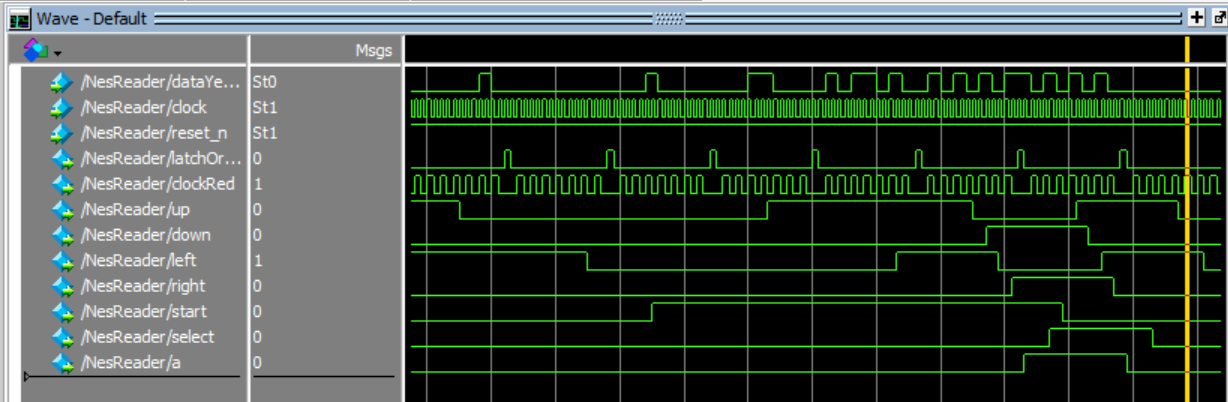
\includegraphics[width=0.8 \linewidth]{images/NESSIM.png}
    \caption{"Button Mashing" on the NES}
    \label{nesButtonMash}
\end{figure}

At first, I wanted to test the NES controller reader by just simulating a bunch of random inputs as seen in Figure \ref{nesButtonMash}. I remembered the NES game CONTRA had a cheat code that involved most of the controller's buttons (all but SELECT). The "Contra Code" was then simulated with the following ModelSim macro code.
 
\begin{figure}[H]
    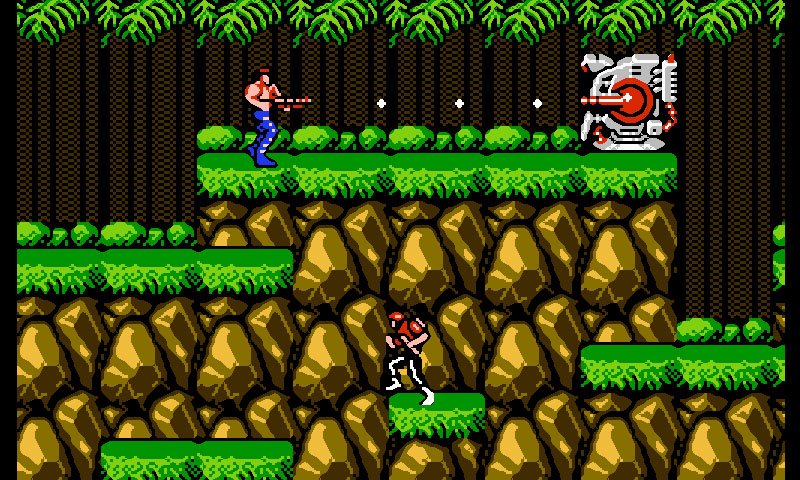
\includegraphics[width=0.8 \linewidth]{images/contra.jpg}
    \caption{CONTRA screenshot}
    \label{contra}
\end{figure}

\begin{figure}[H]
    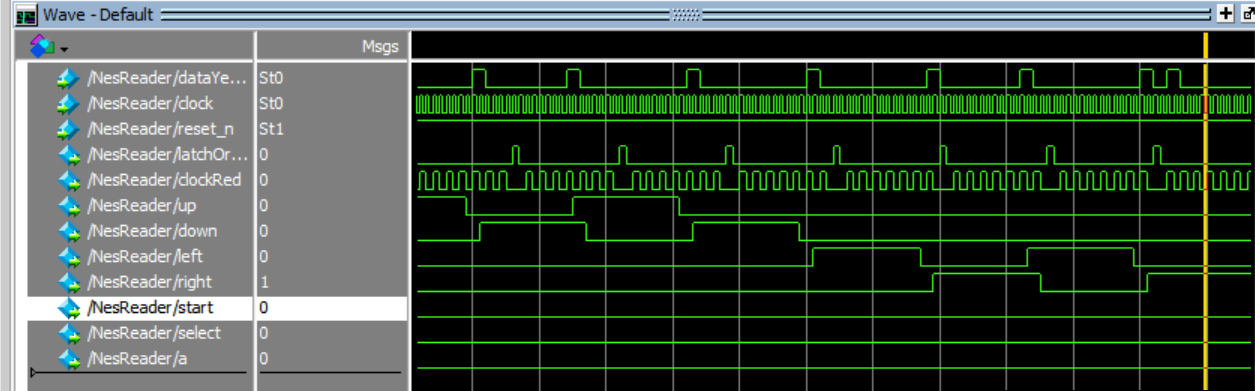
\includegraphics[width=0.8 \linewidth]{images/NESSIMcontra.png}
    \caption{Simulating the "Contra Code" }
    \label{contraSim}
\end{figure}

\begin{verbatim}

force -freeze sim:/NesReader/dataYellow 0 0, 0 {20 ps} , 0 {40 ps} , 0 {60 ps} , 
    1 {80 ps} , 0 {100 ps} , 0 {120 ps} , 0 {140 ps}	#up
force -freeze sim:/NesReader/dataYellow 0 0, 0 {20 ps} , 0 {40 ps} , 0 {60 ps} , 
    0 {80 ps} , 1 {100 ps} , 0 {120 ps} , 0 {140 ps}	#down
force -freeze sim:/NesReader/dataYellow 0 0, 0 {20 ps} , 0 {40 ps} , 0 {60 ps} , 
    1 {80 ps} , 0 {100 ps} , 0 {120 ps} , 0 {140 ps}	#up
force -freeze sim:/NesReader/dataYellow 0 0, 0 {20 ps} , 0 {40 ps} , 0 {60 ps} , 
    0 {80 ps} , 1 {100 ps} , 0 {120 ps} , 0 {140 ps}	#down
force -freeze sim:/NesReader/dataYellow 0 0, 0 {20 ps} , 0 {40 ps} , 0 {60 ps} , 
    0 {80 ps} , 0 {100 ps} , 1 {120 ps} , 0 {140 ps}	#left
force -freeze sim:/NesReader/dataYellow 0 0, 0 {20 ps} , 0 {40 ps} , 0 {60 ps} , 
    0 {80 ps} , 0 {100 ps} , 0 {120 ps} , 1 {140 ps}	#right
force -freeze sim:/NesReader/dataYellow 0 0, 0 {20 ps} , 0 {40 ps} , 0 {60 ps} , 
    0 {80 ps} , 0 {100 ps} , 1 {120 ps} , 0 {140 ps}	#left
force -freeze sim:/NesReader/dataYellow 0 0, 0 {20 ps} , 0 {40 ps} , 0 {60 ps} , 
    0 {80 ps} , 0 {100 ps} , 0 {120 ps} , 1 {140 ps}	#right
force -freeze sim:/NesReader/dataYellow 0 0, 1 {20 ps} , 0 {40 ps} , 0 {60 ps} , 
    0 {80 ps} , 0 {100 ps} , 0 {120 ps} , 0 {140 ps}	#b	
force -freeze sim:/NesReader/dataYellow 1 0, 0 {20 ps} , 0 {40 ps} , 0 {60 ps} , 
    0 {80 ps} , 0 {100 ps} , 0 {120 ps} , 0 {140 ps}	#a
force -freeze sim:/NesReader/dataYellow 0 0, 0 {20 ps} , 0 {40 ps} , 1 {60 ps} , 
    0 {80 ps} , 0 {100 ps} , 0 {120 ps} , 0 {140 ps}	start
\end{verbatim}

\subsubsection{Square Wave Generator}

Our square wave generator module works by receiving a 3-bit data bus and outputs successive octaves of a music note. This module was simply tested by simulating various data inputs on the 3-bit bus. This is pictured in figure \ref{squareSim}.

\begin{figure}[H]
    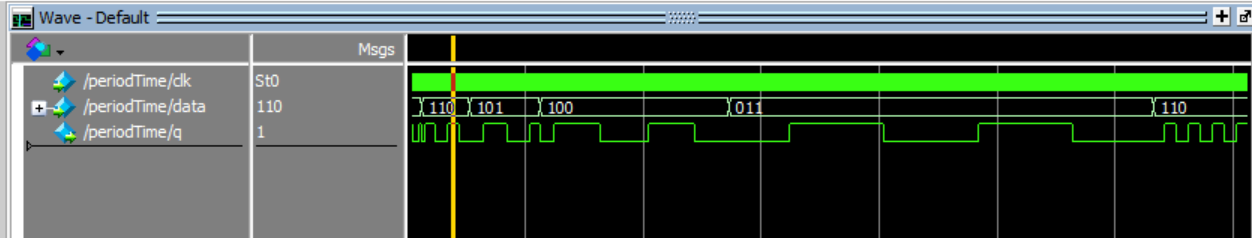
\includegraphics[width=0.8 \linewidth]{images/squareSim.png}
    \caption{Simulating button inputs to control the square wave oscillator}
    \label{squareSim}
\end{figure}

\subsubsection{VGA Output}

\begin{figure}[H]
    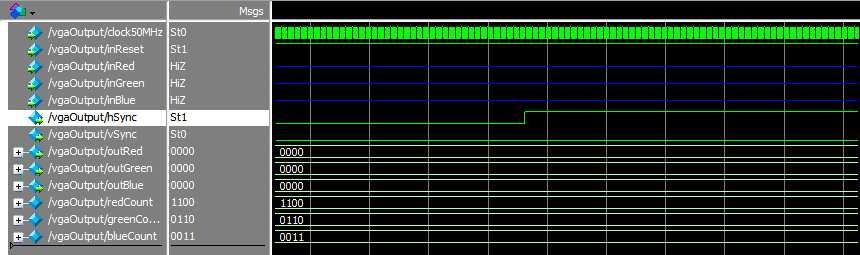
\includegraphics[width=0.8 \linewidth]{images/vgaOutputSim.png}
    \caption{Simulating inputs to the VGA output}
    \label{vgaOutputSim}
\end{figure}

Do File:

\begin{Verbatim}

add wave -position insertpoint sim:/periodTime/*
force -freeze sim:/periodTime/clk 1 0, 0 {5 ps} -r 10
force -freeze sim:/periodTime/data 00010101 0
run
force -freeze sim:/periodTime/data 0000011111 0
run
force -freeze sim:/periodTime/data 1111111111 0
run
force -freeze sim:/periodTime/data 0000011111 0
run
force -freeze sim:/periodTime/data 0000000111 0
run
force -freeze sim:/periodTime/data 0000100111 0
run

\end{Verbatim}

\subsubsection{VGA hCounterComp}

\begin{figure}[H]
    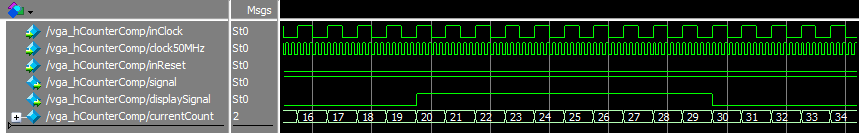
\includegraphics[width=0.8 \linewidth]{images/vgaHCounterCompSim.png}
    \caption{Simulating inputs to the VGA hCounterComp. For this simulation, the range from 20 to 30 is the display range}
    \label{vgaHCounterCompSim}
\end{figure}

Do File:

\begin{Verbatim}
add wave inClock
add wave clock50MHz
add wave inReset
add wave signal
add wave displaySignal
add wave currentCount
force -drive inClock -r 50 0 0, 1 25
force -drive clock50MHz -r 10 0 0, 1 5
force -deposit inReset 1
run
force -deposit inReset 0
run
\end{Verbatim}

\subsubsection{VGA vCounterComp}

\begin{figure}[H]
    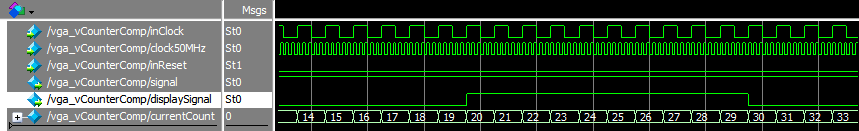
\includegraphics[width=0.8 \linewidth]{images/vgaVCounterCompSim.png}
    \caption{Simulating inputs to the VGA vCounterComp. For this simulation, the range from 20 to 30 is the display range}
    \label{vgaVCounterCompSim}
\end{figure}

Do File:

\begin{Verbatim}
add wave inClock
add wave clock50MHz
add wave inReset
add wave signal
add wave displaySignal
add wave currentCount
force -drive inClock -r 50 0 0, 1 25
force -drive clock50MHz -r 10 0 0, 1 5
force -deposit inReset 1
run
force -deposit inReset 0
run
\end{Verbatim}

\subsubsection{VGA counter}

\begin{figure}[H]
    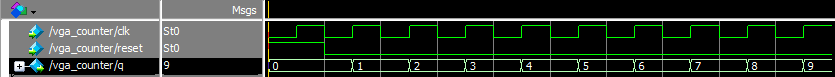
\includegraphics[width=0.8 \linewidth]{images/vgaCounterSim.png}
    \caption{Simulating inputs to the VGA counter}
    \label{vgaCounterSim}
\end{figure}

Do File:

\begin{Verbatim}
add wave clk
add wave reset
add wave q
force -drive clk -r 100 0 0, 1 50
force -deposit reset 1
run
force -deposit reset 0
run
\end{Verbatim}

\subsubsection{VGA displayMux}

\begin{figure}[H]
    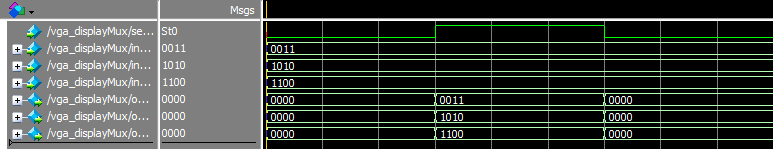
\includegraphics[width=0.8 \linewidth]{images/vgaDisplayMuxSim.png}
    \caption{Simulating inputs to the VGA displayMux}
    \label{vgaDisplayMuxSim}
\end{figure}

Do File:

\begin{Verbatim}
add wave select
add wave inRed
add wave inGreen
add wave inBlue
add wave outRed
add wave outGreen
add wave outBlue
force -deposit inRed 4'b0011
force -deposit inGreen 4'b1010
force -deposit inBlue 4'b1100
force -deposit select 0
run
force -deposit select 1
run
force -deposit select 0
run
\end{Verbatim}

\subsubsection{VGA comparator}

\begin{figure}[H]
    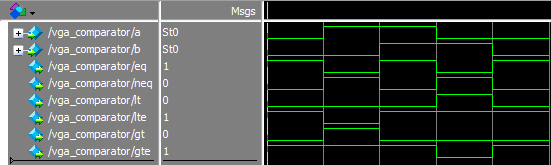
\includegraphics[width=0.8 \linewidth]{images/vgaCompSim.png}
    \caption{Simulating inputs to the VGA comparator}
    \label{vgaCompSim}
\end{figure}

Do file:

\begin{Verbatim}
add wave a
add wave b
add wave eq
add wave neq
add wave gt
add wave gte
add wave lt
add wave lte

force -deposit a 0
force -deposit b 0
run
force -deposit a 1
run
force -deposit b 1
run
force -deposit a 0
run
force -deposit b 0
run
\end{Verbatim}

\subsubsection{VGA synchronizer}

\begin{figure}[H]
    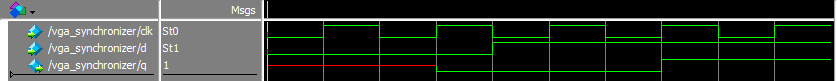
\includegraphics[width=0.8 \linewidth]{images/vgaSyncSim.png}
    \caption{Simulating inputs to the VGA synchronizer module}
    \label{vgaSyncSim}
\end{figure}

Do File:

\begin{Verbatim}
add wave clk
add wave d
add wave q
force -drive clk -r 200 0 0, 1 100
force -deposit d 0
run
force -deposit d 1
run
\end{Verbatim}

\subsubsection{clockDivBy2}

\begin{figure}[H]
    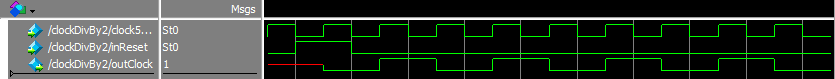
\includegraphics[width=0.8 \linewidth]{images/clockDivBy2Sim.png}
    \caption{Simulating inputs to the clockDivBy2 module}
    \label{clockDivBy2Sim}
\end{figure}

Do File:

\begin{Verbatim}
add wave clock50MHz
add wave inReset
add wave outClock
force -drive clock50MHz -r 100 0 0, 1 50
force -deposit inReset 0
run
force -deposit inReset 1
run
force -deposit inReset 0
run
\end{Verbatim}

\subsubsection{Seven Segment Display: clock_driver}

\begin{figure}[H]
    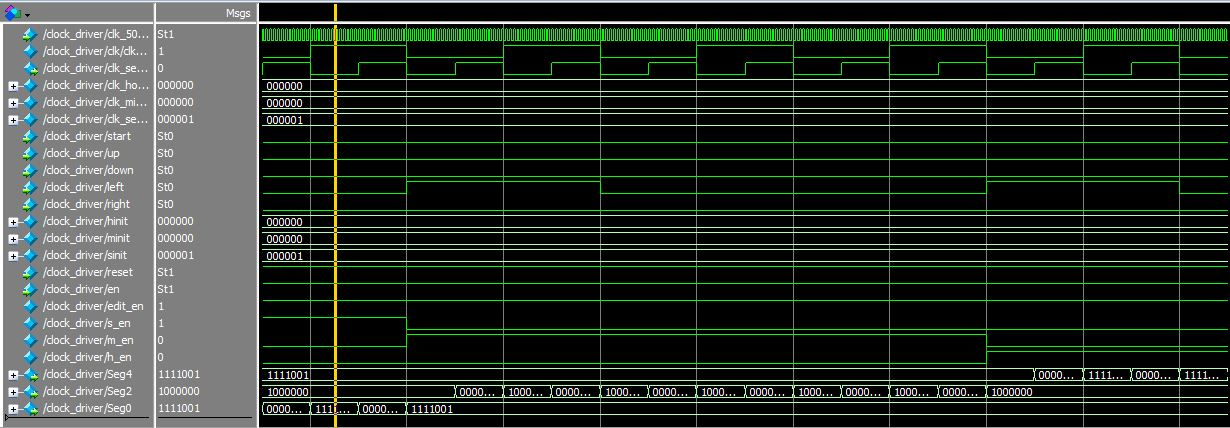
\includegraphics[width=0.8 \linewidth]{images/clock_driver_sim1.JPG}
    \caption{Simulating segments flashing when user is setting values}
    \label{clock_driver_sim1}
\end{figure}
The first simulation ran for the clock_driver module was to check if when the user is setting the seconds, minutes or hours, whichever value they are currently setting will flash (so the user knows which value they are setting. The simulation shows that as the user moves left through the display a corresponding segment from that column flashes at every rising edge of the 2 Hz clock signal.

\begin{figure}[H]
    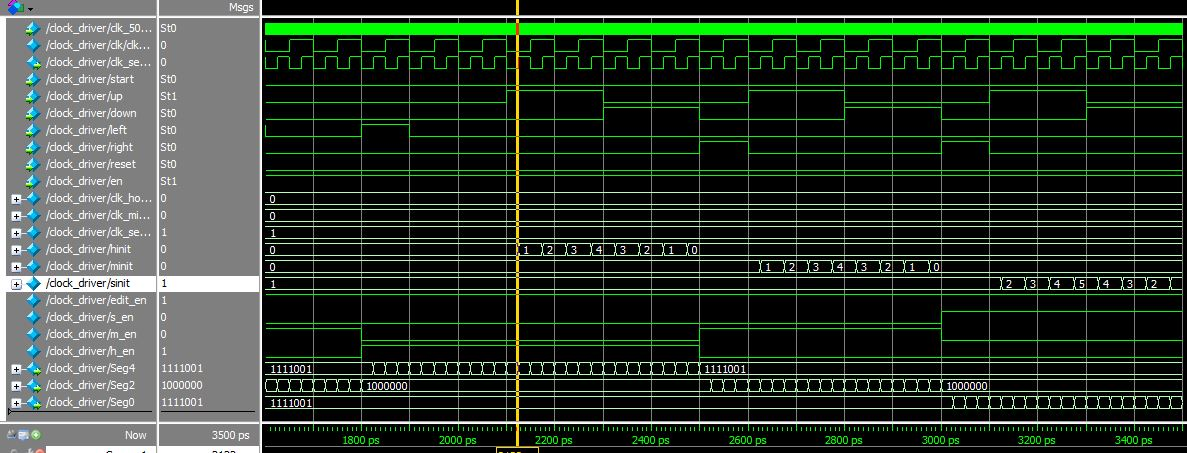
\includegraphics[width=0.8 \linewidth]{images/clock_driver_sim2.JPG}
    \caption{Simulating the user setting the clock}
    \label{clock_driver_sim2}
\end{figure}
The second simulation shows the user moving right through the display, by pulsing the right signal, and adding 1 to to each value at every rising edge of the 2 Hz clock that the signal up is HIGH. Then for each value the signal down is set HIGH, subtracting 1 at the rising edge of each clock.

\begin{figure}[H]
    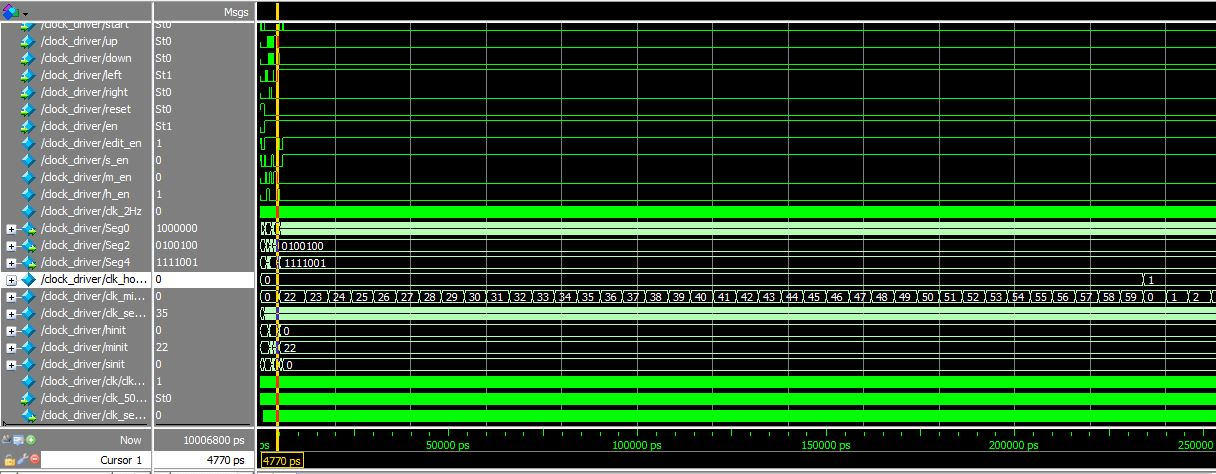
\includegraphics[width=0.8 \linewidth]{images/clock_driver_sim3.JPG}
    \caption{Simulating the setting of values and normal operation of the clock}
    \label{clock_driver_sim3}
\end{figure}
The third and final simulation for this module shows that when the start signal is pulsed while setting the clock, the clock gets set and returns to counting.

Do File:
\begin{Verbatim}
add wave -position insertpoint  \
sim:/clock_driver/clk_seconds
add wave -position insertpoint  \
sim:/clock_driver/hinit
add wave -position insertpoint  \
sim:/clock_driver/minit
add wave -position insertpoint  \
sim:/clock_driver/sinit
add wave -position insertpoint  \
sim:/clock_driver/clk/clk_1Hz
add wave -position insertpoint  \
sim:/clock_driver/clk_50MHz
add wave -position end  sim:/clock_driver/clk_set/clk_2Hz
force clk_set/clk_2Hz 0 0 ps, 1 25 ps -repeat 50 ps
force clk_50MHz 0 0 ps, 1 1 ps -repeat 2 ps
force clk/clk_1Hz 0 0 ps, 1 50 ps -repeat 100 ps
force start 0
force up 0
force down 0
force left 0
force right 0
force reset 1
force en 0
run
force start 1
run
force start 0
run
force start 1
run
force start 0
run
force en 1
force reset 0
run
force start 1
run
force start 0
run
force left 1
run
force left 0
run
force left 1
run
force left 0
run
force up 1
run
force up 0
force down 1
run
force down 0
force right 1
run
force right 0
force up 1
run
force up 0
force down 1
run
force down 0
force right 1
run
force right 0
force up 1
run
force up 0
force down 1
run
force down 0
force left 1
run
force left 0
force up 1
run
force up 0
force left 1
run
force up 1
run
force up 0
force down 1
run
force down 0
force start 1
run
force start 0
run
force start 1
run
force start 0
run 10000 ns

\end{Verbatim}

\subsubsection{Seven Segment Display: clock}

\begin{figure}[H]
    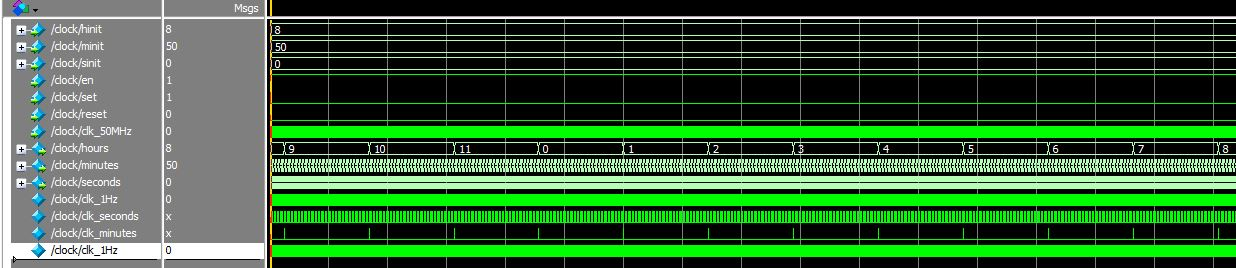
\includegraphics[width=0.8 \linewidth]{images/clock_sim1.JPG}
    \caption{Simulating hours counting and overflowing}
    \label{clock_sim1}
\end{figure}

\begin{figure}[H]
    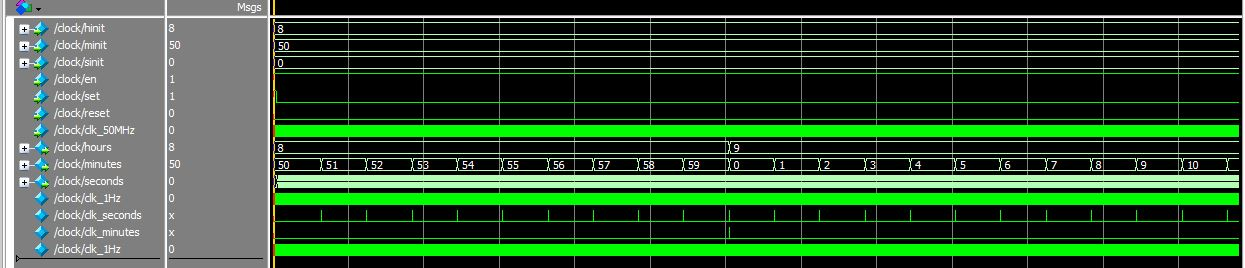
\includegraphics[width=0.8 \linewidth]{images/clock_sim2.JPG}
    \caption{Simulating minutes counting and overflowing}
    \label{clock_sim2}
\end{figure}

\begin{figure}[H]
    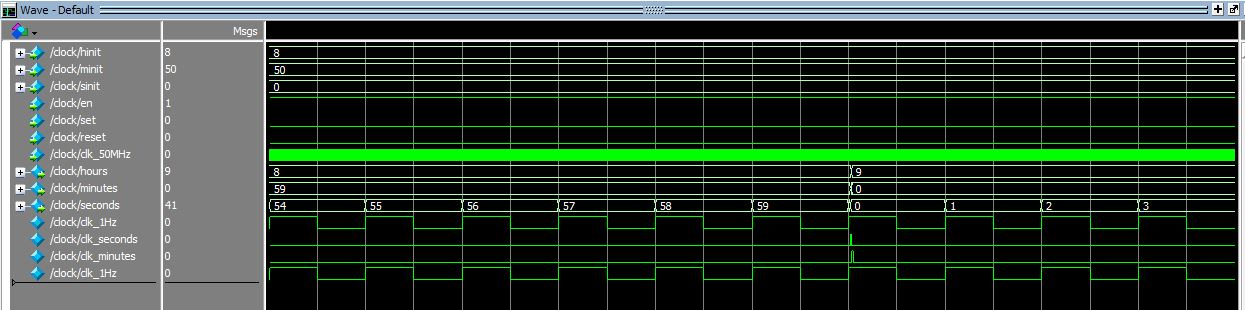
\includegraphics[width=0.8 \linewidth]{images/clock_sim3.JPG}
    \caption{Simulating seconds counting and overflowing}
    \label{clock_sim3}
\end{figure}

Do File:
\begin{Verbatim}
add wave *
force hinit 6'd8
force minit 6'd50
force sinit 0
force en 1
force set 1
force reset 0
force clk_50MHz 0 0 ps, 1 1 ps -repeat 2 ps
add wave -position end  sim:/clock/clk_1Hz
force clk_1Hz 0 0 ps, 1 100 ps -repeat 200 ps
force set 0
run 100000 ns

\end{Verbatim}

\subsubsection{Seven Segment Display: parser}
\begin{figure}[H]
    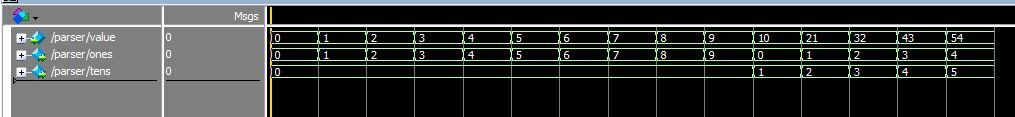
\includegraphics[width=0.8 \linewidth]{images/parser_sim.JPG}
    \caption{Simulating the parser that parses the values of the clock to be displayed}
    \label{parser_sim}
\end{figure}
The parser was simulated for all values but for ease of viewing, this simulation shows all possible outputs for ones and tens once.

Do File:
\begin{Verbatim}
add wave *
force value 8'd0
run
force value 8'd1
run
force value 8'd2
run
force value 8'd3
run
force value 8'd4
run
force value 8'd5
run
force value 8'd6
run
force value 8'd7
run
force value 8'd8
run
force value 8'd9
run
force value 8'd10
run
force value 8'd21
run
force value 8'd32
run
force value 8'd43
run
force value 8'd54
run

\end{Verbatim}

\subsubsection{Seven Segment Display: seven_seg_driver}
\begin{figure}[H]
    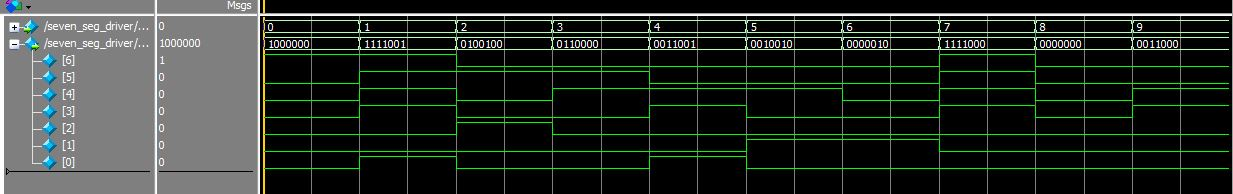
\includegraphics[width=0.8 \linewidth]{images/seven_segment_driver_sim.JPG}
    \caption{Simulating all possible outputs for the seven segment display decoder}
    \label{seven_segment_driver_sim}
\end{figure}

Do File:
\begin{Verbatim}
add wave *
force data 6'd0
run
force data 6'd1
run
force data 6'd2
run
force data 6'd3
run
force data 6'd4
run
force data 6'd5
run
force data 6'd6
run
force data 6'd7
run
force data 6'd8
run
force data 6'd9
run

\end{Verbatim}

\subsubsection{Seven Segment Display: clk_divider.JPG}
\begin{figure}[H]
    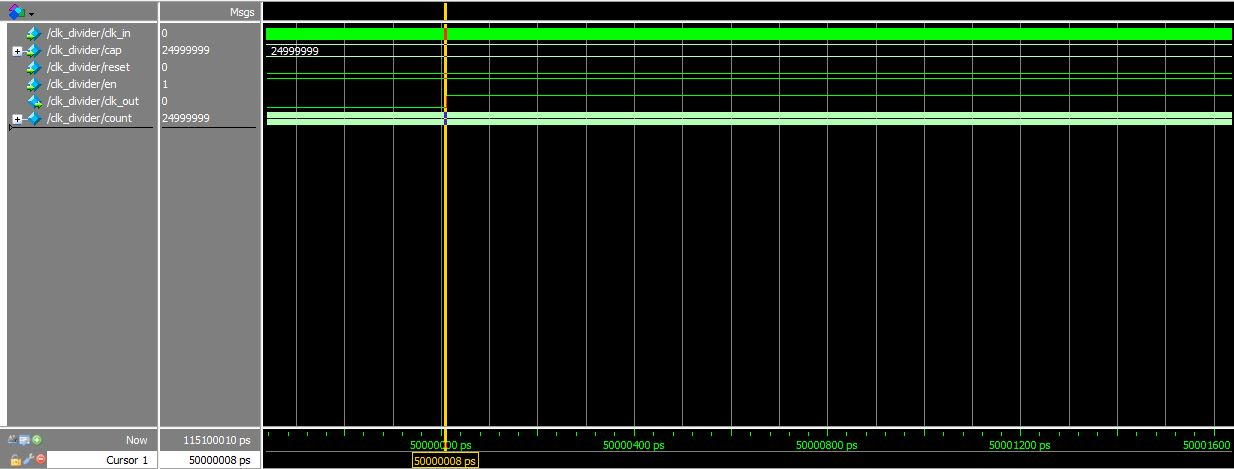
\includegraphics[width=0.8 \linewidth]{images/clk_divider_sim}
    \caption{Simulating the clk_divider toggling the clk_out output at the specified cap}
    \label{clk_divider_sim}
\end{figure}

Do File:
\begin{Verbatim}
force clk_in 0 0 ps, 1 1 ps -repeat 2 ps
add wave *
force cap 26'd24999999
force reset 1
run 10 ps
force reset 0
run 100000 ns

\end{Verbatim}

\subsubsection{Seven Segment Display: clk_counter.JPG}
\begin{figure}[H]
    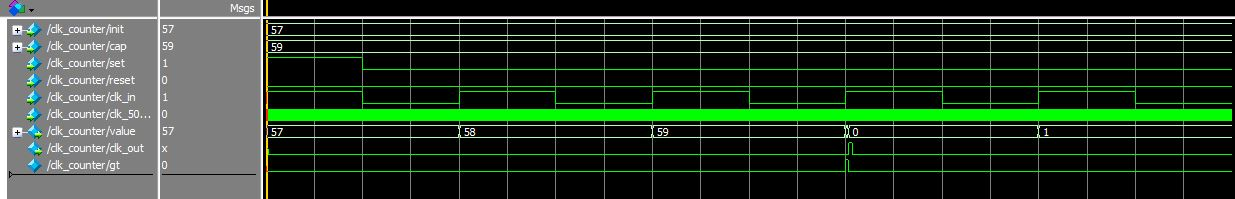
\includegraphics[width=0.8 \linewidth]{images/clk_counter_sim}
    \caption{Simulating the clk_counter resetting after 59 counts}
    \label{clk_counter_sim}
\end{figure}

Do File:
\begin{Verbatim}
add wave *
force init 6'd57
force cap 6'd59
force set 1
force reset 0
force clk_50MHz 0 0 ps, 1 1 ps -repeat 2 ps
force clk_in 0 0 ps, 1 100 ps -repeat 200 ps
force set 0
run 900 ps

\end{Verbatim}

\subsubsection{Seven Segment Display: counter}
\begin{figure}[H]
    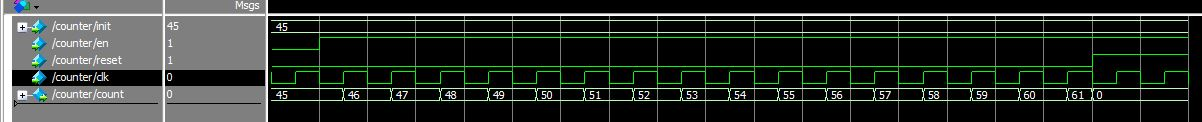
\includegraphics[width=0.8 \linewidth]{images/counter_sim.JPG}
    \caption{Simulating the counter module counting from an initial value and resetting}
    \label{counter_sim}
\end{figure}

Do File:
\begin{Verbatim}
add wave *
force init 6'd45
force en 0
force reset 0
force clk 0 0 ps, 1 25 ps -repeat 50 ps
run
force en 1
run 800 ps
force reset 1
run

\end{Verbatim}

\subsubsection{Seven Segment Display: comp}
\begin{figure}[H]
    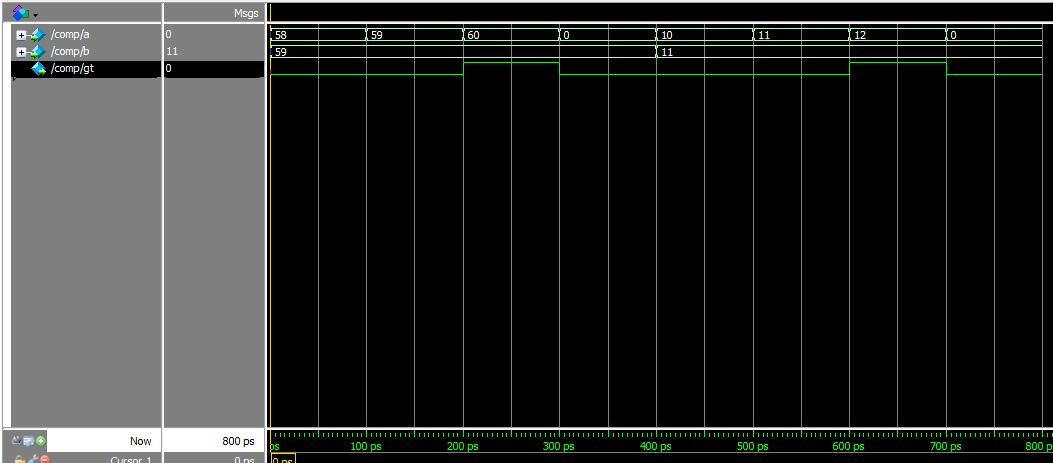
\includegraphics[width=0.8 \linewidth]{images/comp_sim.JPG}
    \caption{Simulating the comparator with a gt output of HIGH when input a is greater than input b}
    \label{comp_aim}
\end{figure}

Do File:
\begin{Verbatim}
add wave *

force a 6'd58
force a 6'd59
run

force a 6'd59
run

force a 6'd60
run 

force a 6'd0
run 

force a 6'd10
force b 6'd11
run

force a 6'd11
run

force a 6'd12
run

force a 6'd0
run
\end{Verbatim}

\subsubsection{Seven Segment Display: sync}
\begin{figure}[H]
    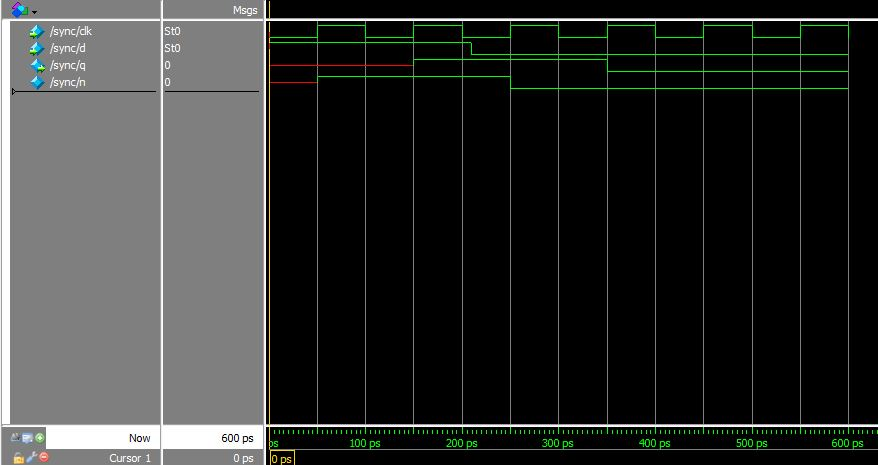
\includegraphics[width=0.8 \linewidth]{images/sync_sim.JPG}
    \caption{Simulating the input in the synchronizer propagating to the output at the rising edge of the clock}
    \label{sync_sim}
\end{figure}

Do File:
\begin{Verbatim}
add wave *
force clk 0 0 ps, 1 50 ps -repeat 100 ps
force d 1
run
run
run 10 ps
force d 0
run 90 ps
run
run
run
\end{Verbatim}

\subsubsection{Seven Segment Display: clock_set.JPG}
\begin{figure}[H]
    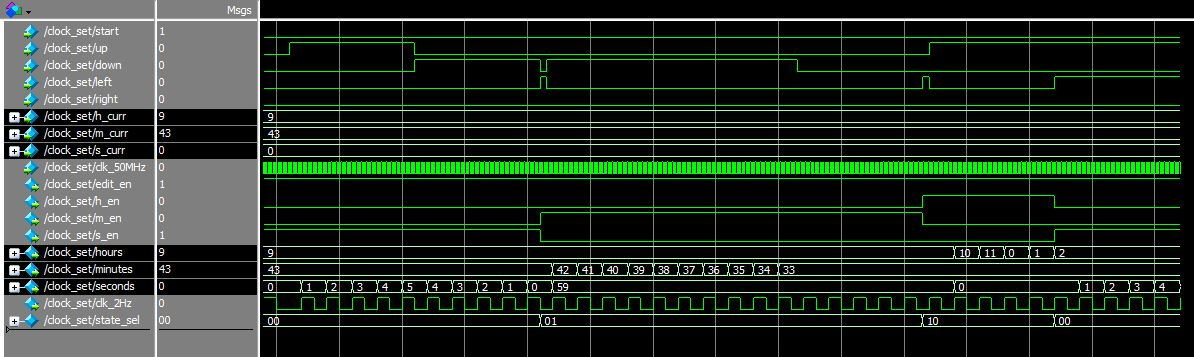
\includegraphics[width=0.8 \linewidth]{images/clock_set_sim}
    \caption{Simulating the clock_set module letting the user navigate through the clock and set each value}
    \label{clock_set_sim}
\end{figure}

Do File:
\begin{Verbatim}
add wave *
force start 0
force up 0
force down 0
force left 0
force right 0
force h_curr 6'd9
force m_curr 6'd43
force s_curr 6'd0
force clk_50MHz 0 0 ps, 1 1 ps -repeat 2 ps
force clk_2Hz 0 0 ps, 1 50 ps -repeat 100 ps
run
force start 1
run 10 ps
force start 0
run
force up 1
force clk_2Hz 0 0 ps, 1 10 ps -repeat 20 ps
run
force up 0
force down 1
run
force down 0
force left 1
run 5 ps
force left 0
force down 1
run
run
force down 0
run
force left 1
run 5 ps
force left 0
force up 1
run
force left 1
run
\end{Verbatim}

\subsubsection{Seven Segment Display: clk_column_sel.JPG}
\begin{figure}[H]
    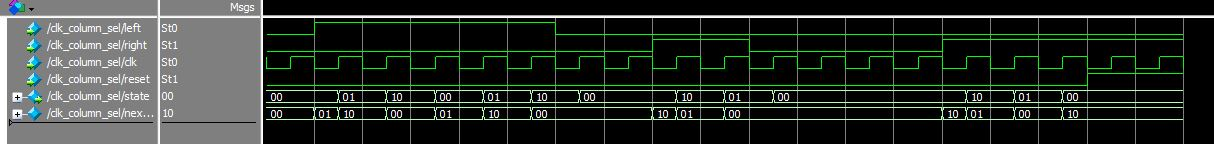
\includegraphics[width=0.8 \linewidth]{images/clk_column_sel_sim}
    \caption{Simulating the clk_column_sel module that lets the user navigate through seconds, minutes and hours}
    \label{clk_column_sel_sim}
\end{figure}

Do File:
\begin{Verbatim}
add wave *
force start 0
force up 0
force down 0
force left 0
force right 0
force h_curr 6'd9
force m_curr 6'd43
force s_curr 6'd0
force clk_50MHz 0 0 ps, 1 1 ps -repeat 2 ps
force clk_2Hz 0 0 ps, 1 50 ps -repeat 100 ps
run
force start 1
run 10 ps
force start 0
run
force up 1
force clk_2Hz 0 0 ps, 1 10 ps -repeat 20 ps
run
force up 0
force down 1
run
force down 0
force left 1
run 5 ps
force left 0
force down 1
run
run
force down 0
run
force left 1
run 5 ps
force left 0
force up 1
run
force left 1
run
\end{Verbatim}

\subsubsection{Seven Segment Display: updowncounter}
\begin{figure}[H]
    \includegraphics[width=0.8 \linewidth]{images/updowncounter_sim.JPG}
    \caption{Simulating the updowncounter module which can count up or down, and overflow both ways}
    \label{updowncounter_sim}
\end{figure}

Do File:
\begin{Verbatim}
force clk_in 0 0 ps, 1 25 ps -repeat 50 ps
force up 0
force down 0
add wave *
force en 1
force reset 1
force cap 6'd59
force init 6'd45
run
force reset 0
force up 1
run 1100 ps
force up 0
force down 1
run 600 ps
\end{Verbatim}

%\includepdf[page=-]{Ch3Example}

\end{document}
